\documentclass[onecolumn, compsoc,12pt]{IEEEtran}
\usepackage{paralist}
\usepackage{enumitem}
\usepackage{etex}
\usepackage{amssymb,amsfonts,amsmath,amsthm}
\usepackage{graphicx}
\usepackage{booktabs}
\usepackage[usenames,x11names, dvipsnames, svgnames]{xcolor}
\usepackage{amsmath,amssymb}
\usepackage{dsfont}
\usepackage{amsfonts}
\usepackage{mathrsfs}
\usepackage{texshade}
\usepackage{hyperref}
\hypersetup{
  colorlinks=true,
  linkcolor=black,
  citecolor=blue,
  filecolor=black,
  urlcolor=DodgerBlue4,
  breaklinks=false,
  % linkbordercolor=red,% hyperlink borders will be red
  % pdfborderstyle={/S/U/W 1}% border style will be underline of width 1pt
}
\usepackage{array}
\usepackage{xr}
\usepackage{verbatim}
\usepackage{multirow}
\usepackage{longtable}
\usepackage{tikz-network}
\usepackage[T1,euler-digits]{eulervm}
\usepackage{times}
% \usepackage{pxfonts}
\usepackage{tikz}
\usepackage{pgfplots}
\usetikzlibrary{shapes,calc,shadows,fadings,arrows,decorations.pathreplacing,automata,positioning}
\usetikzlibrary{external}
\usetikzlibrary{decorations.text}
\usepgfplotslibrary{colorbrewer} 
\usepgfplotslibrary{statistics}

\tikzexternalize[prefix=./Figures/External/]% activate externalization!
\tikzexternaldisable
% \addtolength{\voffset}{.1in}  
\usepackage{geometry}
\geometry{letterpaper, left=.6in,right=.6in,top=.5in,bottom=0.7in}

%\addtolength{\textwidth}{-.1in}    
%\addtolength{\hoffset}{.05in}    
%\addtolength{\textheight}{.1in}    
%\addtolength{\footskip}{0in}    
\usepackage{rotating}
\definecolor{nodecol}{RGB}{240,240,220}
\definecolor{nodeedge}{RGB}{240,240,225}
\definecolor{edgecol}{RGB}{130,130,130}
\tikzset{%
  fshadow/.style={      preaction={
      fill=black,opacity=.3,
      path fading=circle with fuzzy edge 20 percent,
      transform canvas={xshift=1mm,yshift=-1mm}
    }} 
}
\usetikzlibrary{pgfplots.dateplot}
\usetikzlibrary{patterns}
\usetikzlibrary{decorations.markings}
\usepackage{fancyhdr}
\usepackage{mathtools}
\usepackage{datetime}
\usepackage{comment}
%% ## Equation Space Control---------------------------
\def\EQSP{3pt}
\newcommand{\mltlne}[2][\EQSP]{\begingroup\setlength\abovedisplayskip{#1}\setlength\belowdisplayskip{#1}\begin{equation}\begin{multlined} #2 \end{multlined}\end{equation}\endgroup\noindent}
\newcommand{\cgather}[2][\EQSP]{\begingroup\setlength\abovedisplayskip{#1}\setlength\belowdisplayskip{#1}\begin{gather} #2 \end{gather}\endgroup\noindent}
\newcommand{\cgathers}[2][\EQSP]{\begingroup\setlength\abovedisplayskip{#1}\setlength\belowdisplayskip{#1}\begin{gather*} #2 \end{gather*}\endgroup\noindent}
\newcommand{\calign}[2][\EQSP]{\begingroup\setlength\abovedisplayskip{#1}\setlength\belowdisplayskip{#1}\begin{align} #2 \end{align}\endgroup\noindent}
\newcommand{\caligns}[2][\EQSP]{\begingroup\setlength\abovedisplayskip{#1}\setlength\belowdisplayskip{#1}\begin{align*} #2 \end{align*}\endgroup\noindent}
\newcommand{\mnp}[2]{\begin{minipage}{#1}#2\end{minipage}} 
%% COLOR DEFS------------------------------------------
\newtheorem{thm}{Theorem}
\newtheorem{cor}{Corollary}
\newtheorem{lem}{Lemma}
\newtheorem{prop}{Proposition}
\newtheorem{defn}{Definition}
\newtheorem{exmpl}{Example}
\newtheorem{rem}{Remark}
\newtheorem{notn}{Notation}
%% ------------PROOF INCLUSION -----------------
\def\NOPROOF{Proof omitted.}
\newif\ifproof
\prooffalse % or \draftfalse
\newcommand{\Proof}[1]{
  \ifproof
  \begin{IEEEproof}
    #1\end{IEEEproof}
  \else
  \NOPROOF
  \fi
}
%% ------------ -----------------
\newcommand{\DETAILS}[1]{#1}
%% ------------ -----------------
% color commands------------------------
\newcommand{\etal}{\textit{et} \mspace{3mu} \textit{al.}}
% \renewcommand{\algorithmiccomment}[1]{$/** $ #1 $ **/$}
\newcommand{\vect}[1]{\textbf{\textit{#1}}}
\newcommand{\figfont}{\fontsize{8}{8}\selectfont\strut}
\newcommand{\hlt}{ \bf \sffamily \itshape\color[rgb]{.1,.2,.45}}
\newcommand{\pitilde}{\widetilde{\pi}}
\newcommand{\Pitilde}{\widetilde{\Pi}}
\newcommand{\bvec}{\vartheta}
\newcommand{\algo}{\textrm{\bf\texttt{GenESeSS}}\xspace}
\newcommand{\xalgo}{\textrm{\bf\texttt{xGenESeSS}}\xspace}
\newcommand{\FNTST}{\bf }
\newcommand{\FNTED}{\color{darkgray} \scriptsize $\phantom{.}$}
\renewcommand{\baselinestretch}{.9}
\newcommand{\sync}{\otimes}
\newcommand{\psync}{\hspace{3pt}\overrightarrow{\hspace{-3pt}\sync}}
% \newcommand{\psync}{\raisebox{-4pt}{\begin{tikzpicture}\node[anchor=south] (A) {$\sync$};
%   \draw [->,>=stealth] ([yshift=-2pt, xshift=2pt]A.north west) -- ([yshift=-2pt]A.north east); %\end{tikzpicture}}}
\newcommand{\base}[1]{\llbracket #1 \rrbracket}
\newcommand{\nst}{\textrm{\sffamily\textsc{Numstates}}}
\newcommand{\HA}{\boldsymbol{\mathds{H}}}
\newcommand{\eqp}{ \vartheta }
\newcommand{\entropy}[1]{\boldsymbol{h}\left ( #1 \right )}
\newcommand{\norm}[1]{\left\lVert #1 \right\rVert}%
\newcommand{\abs}[1]{\left\lvert #1 \right\rvert}%
\newcommand{\absB}[1]{\big\lvert #1 \big\rvert}%
% #############################################################
% #############################################################
% PREAMBLE ####################################################
% #############################################################
% #############################################################
% \usepackage{pnastwoF}      
\DeclareMathOperator*{\argmax}{argmax}
\DeclareMathOperator*{\argmin}{arg\,min}
\DeclareMathOperator*{\expect}{\mathbf{E}}
\DeclareMathOperator*{\var}{\mathbf{Var}}

\newcommand{\ND}{ \mathcal{N}  }
\usepackage[linesnumbered,ruled,vlined,noend]{algorithm2e}
\newcommand{\captionN}[1]{\caption{\color{darkgray} \sffamily \fontsize{9}{10}\selectfont #1  }}
\newcommand{\btl}{\ \textbf{\small\sffamily bits/letter}}
%\usepackage{txfonts}
%%% \usepackage{ccfonts}
%%% save defaults
%\renewcommand{\rmdefault}{phv} % Arial
%\renewcommand{\sfdefault}{phv} % Arial
%\edef\keptrmdefault{\rmdefault}
%\edef\keptsfdefault{\sfdefault}
%\edef\keptttdefault{\ttdefault}

% \usepackage{kerkis}
%\usepackage[OT1]{fontenc}
%\usepackage{concmath}
% \usepackage[T1]{eulervm} 
% \usepackage[OT1]{fontenc}
%%% restore defaults
%\edef\rmdefault{\keptrmdefault}
%\edef\sfdefault{\keptsfdefault}
%\edef\ttdefault{\keptttdefault}
\tikzexternalenable
% ##########################################################
\tikzfading[name=fade out,
inner color=transparent!0,
outer color=transparent!100]
% ###################################
\newcommand{\xtitaut}[2]{
  \noindent\mnp{\textwidth}{
    \mnp{\textwidth}{\raggedright\Huge \bf \sffamily #1}

    \vskip 1em

    {\bf \sffamily #2}
  }
  \vskip 2em
}
% ###################################
% ###################################
\tikzset{wiggle/.style={decorate, decoration={random steps, amplitude=10pt}}}
\usetikzlibrary{decorations.pathmorphing}
\pgfdeclaredecoration{Snake}{initial}
{
  \state{initial}[switch if less than=+.625\pgfdecorationsegmentlength to final,
  width=+.3125\pgfdecorationsegmentlength,
  next state=down]{
    \pgfpathmoveto{\pgfqpoint{0pt}{\pgfdecorationsegmentamplitude}}
  }
  \state{down}[switch if less than=+.8125\pgfdecorationsegmentlength to end down,
  width=+.5\pgfdecorationsegmentlength,
  next state=up]{
    \pgfpathcosine{\pgfqpoint{.25\pgfdecorationsegmentlength}{-1\pgfdecorationsegmentamplitude}}
    \pgfpathsine{\pgfqpoint{.25\pgfdecorationsegmentlength}{-1\pgfdecorationsegmentamplitude}}
  }
  \state{up}[switch if less than=+.8125\pgfdecorationsegmentlength to end up,
  width=+.5\pgfdecorationsegmentlength,
  next state=down]{
    \pgfpathcosine{\pgfqpoint{.25\pgfdecorationsegmentlength}{\pgfdecorationsegmentamplitude}}
    \pgfpathsine{\pgfqpoint{.25\pgfdecorationsegmentlength}{\pgfdecorationsegmentamplitude}}
  }
  \state{end down}[width=+.3125\pgfdecorationsegmentlength,
  next state=final]{
    \pgfpathcosine{\pgfqpoint{.15625\pgfdecorationsegmentlength}{-.5\pgfdecorationsegmentamplitude}}
    \pgfpathsine{\pgfqpoint{.15625\pgfdecorationsegmentlength}{-.5\pgfdecorationsegmentamplitude}}
  }
  \state{end up}[width=+.3125\pgfdecorationsegmentlength,
  next state=final]{
    \pgfpathcosine{\pgfqpoint{.15625\pgfdecorationsegmentlength}{.5\pgfdecorationsegmentamplitude}}
    \pgfpathsine{\pgfqpoint{.15625\pgfdecorationsegmentlength}{.5\pgfdecorationsegmentamplitude}}
  }
  \state{final}{\pgfpathlineto{\pgfpointdecoratedpathlast}}
}
% ###################################
% ###################################
\newcolumntype{L}[1]{>{\rule{0pt}{2ex}\raggedright\let\newline\\\arraybackslash\hspace{0pt}}m{#1}}
\newcolumntype{C}[1]{>{\rule{0pt}{2ex}\centering\let\newline\\\arraybackslash\hspace{0pt}}m{#1}}
\newcolumntype{R}[1]{>{\rule{0pt}{2ex}\raggedleft\let\newline\\\arraybackslash\hspace{0pt}}m{#1}}



% ################################################
% ################################################
% ################################################
% ################################################
\def\DISCLOSURE#1{\def\disclosure{#1}}
\DISCLOSURE{\raisebox{15pt}{$\phantom{XxxX}$This sheet contains proprietary information 
    not to be released to third parties except for the explicit purpose of evaluation.}
}
% ####################################
\newcommand{\set}[1]{\left\{ #1 \right\}}
\newcommand{\paren}[1]{\left( #1 \right)}
\newcommand{\bracket}[1]{\left[ #1 \right]}
% \newcommand{\norm}[1]{\left\Vert #1 \right\Vert}
\newcommand{\nrm}[1]{\left\llbracket{#1}\right\rrbracket}
\newcommand{\parenBar}[2]{\paren{#1\,{\left\Vert\,#2\right.}}}
\newcommand{\parenBarl}[2]{\paren{\left.#1\,\right\Vert\,#2}}
\newcommand{\ie}{$i.e.$\xspace}
\newcommand{\addcitation}{\textcolor{black!50!red}{\textbf{ADD CITATION}}}
\newcommand{\subtochange}[1]{{\color{black!50!green}{#1}}}
\newcommand{\tobecompleted}{{\color{black!50!red}TO BE COMPLETED.}}


\newcommand{\pIn}{\mathscr{P}_{\textrm{in}}}
\newcommand{\pOut}{\mathscr{P}_{\textrm{out}}}
\newcommand{\aIn}[1][\Sigma]{#1_{\textrm{in}}}
\newcommand{\aOut}[1][\Sigma]{#1_{\textrm{out}}}
\newcommand{\xin}[1]{#1_{\textrm{in}}}
\newcommand{\xout}[1]{#1_{\textrm{out}}}

\newcommand{\R}{\mathbb{R}} % Set of real numbers
\newcommand{\F}[1][]{\mathcal{F}_{#1}}
\newcommand{\SR}{\mathcal{S}} % Semiring of sets
\newcommand{\RR}{\mathcal{R}} % Ring of sets
\newcommand{\N}{\mathbb{N}} % Set of natural numbers (0 included)


\newcommand{\Pp}[1][n]{\mathscr{P}^+_{#1}}
\renewcommand{\entropy}[1]{\boldsymbol{h}\left ( #1 \right )}



\makeatletter
\pgfdeclarepatternformonly[\hatchdistance,\hatchthickness]{flexible hatch}
{\pgfqpoint{0pt}{0pt}}
{\pgfqpoint{\hatchdistance}{\hatchdistance}}
{\pgfpoint{\hatchdistance-1pt}{\hatchdistance-1pt}}%
{
  \pgfsetcolor{\tikz@pattern@color}
  \pgfsetlinewidth{\hatchthickness}
  \pgfpathmoveto{\pgfqpoint{0pt}{0pt}}
  \pgfpathlineto{\pgfqpoint{\hatchdistance}{\hatchdistance}}
  \pgfusepath{stroke}
}
\makeatother

\pgfdeclarepatternformonly{north east lines wide}%
{\pgfqpoint{-1pt}{-1pt}}%
{\pgfqpoint{10pt}{10pt}}%
{\pgfqpoint{9pt}{9pt}}%
{
  \pgfsetlinewidth{0.7pt}
  \pgfpathmoveto{\pgfqpoint{0pt}{0pt}}
  \pgfpathlineto{\pgfqpoint{9.1pt}{9.1pt}}
  \pgfusepath{stroke}
}

\pgfdeclarepatternformonly{north west lines wide}%
{\pgfqpoint{-1pt}{-1pt}}%
{\pgfqpoint{10pt}{10pt}}%
{\pgfqpoint{9pt}{9pt}}%
{
  \pgfsetlinewidth{0.7pt}
  \pgfpathmoveto{\pgfqpoint{0pt}{9pt}}
  \pgfpathlineto{\pgfqpoint{9.1pt}{-0.1pt}}
  \pgfusepath{stroke}
}
\makeatletter

\pgfdeclarepatternformonly[\hatchdistance,\hatchthickness]{flexible hatchB}
{\pgfqpoint{0pt}{\hatchdistance}}
{\pgfqpoint{\hatchdistance}{0pt}}
{\pgfpoint{1pt}{\hatchdistance-1pt}}%
{
  \pgfsetcolor{\tikz@pattern@color}
  \pgfsetlinewidth{\hatchthickness}
  \pgfpathmoveto{\pgfqpoint{0pt}{\hatchdistance}}
  \pgfpathlineto{\pgfqpoint{\hatchdistance}{0pt}}
  \pgfusepath{stroke}
}    \makeatother


\def\TPR{\textrm{TPR}\xspace}
\def\TNR{\textrm{TNR}\xspace}
\def\FPR{\textrm{FPR}\xspace}
\def\PPV{\textrm{PPV}\xspace}

\usetikzlibrary{arrows.meta}
\usetikzlibrary{decorations.pathreplacing,shapes.misc}
\usepgfplotslibrary{fillbetween}
%usepackage{tikz-network}
\usetikzlibrary{shapes.geometric}
\usetikzlibrary{math}
\usepgfplotslibrary{colorbrewer} 

\usepackage{textcomp}
\usepackage{colortbl}
\usepackage{array}
\usepackage{courier} 
\usepackage{wrapfig}
\usepackage{pifont}
\usetikzlibrary{chains,backgrounds}
\usetikzlibrary{intersections}
\usetikzlibrary{pgfplots.groupplots}
\usepgfplotslibrary{fillbetween} 
\usetikzlibrary{arrows.meta}
\usepackage{pgfplotstable}
\usepackage[super,compress,sort,comma]{natbib}
%\usepackage{natbib}
\usepackage{setspace}
\usetikzlibrary{math}
\usetikzlibrary{matrix}
\usepackage{xstring}
\usepackage{xspace}
\usepackage{flushend}
\makeatletter
\renewcommand\section{\@startsection {section}{1}{\z@}%
  {-2ex \@plus -1ex \@minus -.2ex}%
  {1ex \@plus.1ex}%
  {\Large\bfseries\scshape}}
\renewcommand\subsection{\@startsection {subsection}{1}{\z@}%
  {-2ex \@plus -.25ex \@minus -.2ex}%
  {0.1ex \@plus.0ex}%
  {\fontsize{11}{10}\selectfont\bfseries\sffamily\color{black}}}
\renewcommand\subsubsection{\@startsection {subsubsection}{1}{\z@}%
  {0ex \@plus -.5ex \@minus -.2ex}%
  {0.0ex \@plus.5ex}%
  {\bfseries\itshape\sffamily\color{darkgray}}}
\renewcommand\paragraph{\@startsection {paragraph}{1}{\z@}%
  {-.2ex \@plus -.5ex \@minus -.2ex}%
  {0.0ex \@plus.5ex}%
  {\fontsize{9}{9}\selectfont\itshape\sffamily\color{darkgray}}}
       
%\renewcommand{\thesubsection}{\thesection.\arabic{subsection}}
\renewcommand{\thesubsectiondis}{\arabic{subsection}.}
\renewcommand{\thesectiondis}{\arabic{section}.}
\renewcommand{\thesection}{\arabic{section}}

\renewcommand{\thetable}{\arabic{table}}

\makeatother
\makeatletter
\pgfdeclareradialshading[tikz@ball]{ball}{\pgfqpoint{-10bp}{10bp}}{%
  color(0bp)=(tikz@ball!30!white);
  color(9bp)=(tikz@ball!75!white);
  color(18bp)=(tikz@ball!90!black);
  color(25bp)=(tikz@ball!70!black);
  color(50bp)=(black)}
\makeatother
%\newcommand{\tball}[1][CadetBlue4]{${\color{#1}\Large\boldsymbol{\blacksquare}}$}
\renewcommand{\baselinestretch}{1}
%\renewcommand{\captionN}[1]{\caption{\color{CadetBlue4!50!black} \sffamily \fontsize{9}{10}\selectfont #1  }}
\tikzexternaldisable 
\parskip=6pt
\parindent=0pt
%\newcommand{\Mark}[1]{\textsuperscript{#1}}
\pagestyle{fancy}

\newcounter{Dcounter}
\setcounter{Dcounter}{1}
\newcommand{\DQS}[1]{\marginpar{\tikzexternaldisable \tikz{\node[rounded corners=5pt,draw=none,thick,fill=black!10,font=\sffamily\fontsize{7}{8}\selectfont] {\mnp{.45in} {\color{Red3}\raggedright  \#\theDcounter.~#1}}; }}\stepcounter{Dcounter}\xspace}

\newcommand{\qn}[1][i]{\Phi_{#1}}
\newcommand{\D}[1][i]{\mathscr{D}\left ( {\Sigma_#1} \right ) }
\newcommand{\Dx}{\mathscr{D}}
\def\J{\mathds{J}}
\def\M{\omega}
\def\N{\mathds{N}}
\newcommand{\cp}[1][P]{\langle #1 \rangle}
\newcommand{\mem}[1]{\M_{#1}}


\makeatletter
\newcommand\transformxdimension[1]{
    \pgfmathparse{((#1/\pgfplots@x@veclength)+\pgfplots@data@scale@trafo@SHIFT@x)/10^\pgfplots@data@scale@trafo@EXPONENT@x}
}
\newcommand\transformydimension[1]{
    \pgfmathparse{((#1/\pgfplots@y@veclength)+\pgfplots@data@scale@trafo@SHIFT@y)/10^\pgfplots@data@scale@trafo@EXPONENT@y}
}
\makeatother

\parskip=6pt
\parindent=0pt


\pgfplotsset{
    discard if/.style 2 args={
        x filter/.code={
            \edef\tempa{\thisrow{#1}}
            \edef\tempb{#2}
            \ifx\tempa\tempb
                \def\pgfmathresult{inf}
            \fi
        }
    },
    discard if not/.style 2 args={
        x filter/.code={
            \edef\tempa{\thisrow{#1}}
            \edef\tempb{#2}
            \ifx\tempa\tempb
            \else
                \def\pgfmathresult{inf}
            \fi
        }
    }
  }

  %\newcommand{\HLT}[2][Red1]{{\color{#1}#2}}

 % \def\commatonone{\expandafter\zappointzerozero
%    \romannumeral`\^^@}
%\def\zappointzerozero#1.00{\zapcomma#1,!}
%\def\zapcomma#1,#2{#1\ifx!#2\else#2\expandafter\zapcomma\fi}
\def\commatononei#1,{#1}
\def\commatononej#1,#2,{#1#2}
\def\commatonone#1{\expandafter\commatononei#1}
\def\commatononeT#1{\expandafter\commatononej#1}
\newcommand{\Sum} [2] {#1 + #2 = \the\numexpr #1 + #2 \relax \\}


\usepackage{sistyle}
\SIthousandsep{,}

\makeatletter
\newcommand{\limitpages}[1]{
  \gdef\maxpages{#1}%
  \ifx\latex@outputpage\@undefined\relax%
  \global\let\latex@outputpage\@outputpage%
  \fi%
  \gdef\@outputpage{%
    \ifnum\value{page}>\maxpages\relax%
    % Do not output the page
    \else%
    \latex@outputpage%
    \fi%
  }%
}
\makeatother
\newcommand{\note}[1]{{ \itshape \footnotesize \color{Red1}$\medbullet$~ #1}}









\renewcommand{\thesectiondis}{\arabic{section}.}
\renewcommand{\thesubsectiondis}{\Alph{subsection}.}

\makeatletter
\renewcommand\section{\@startsection {section}{1}{\z@}%
  {-1pt \@plus -30ex \@minus 20ex}%
  {.1pt}%
  {\large\bfseries\scshape}}
\renewcommand\subsection{\@startsection {subsection}{2}{\z@}%
  {0ex \@plus -1.75ex \@minus -1.2ex}%
  {0ex \@plus.0ex}%
  {\fontsize{11}{11}\selectfont\bfseries\sffamily\color{black}}}
\renewcommand\subsubsection{\@startsection {section}{1}{\z@}%
  {-.1ex \@plus -.5ex \@minus -.2ex}%
  {0.0ex \@plus.5ex}%
  {\bfseries\sffamily\color{Red4}}}
\renewcommand\paragraph{\@startsection {section}{1}{\z@}%
  {-.1ex \@plus -.5ex \@minus -.2ex}%
  {0.0ex \@plus.5ex}%
  {\fontsize{11}{10}\selectfont\bfseries\itshape\sffamily\color{black}}}
\makeatother


\makeatletter
\pgfdeclareradialshading[tikz@ball]{ball}{\pgfqpoint{-10bp}{10bp}}{%
  color(0bp)=(tikz@ball!30!white);
  color(9bp)=(tikz@ball!75!white);
  color(18bp)=(tikz@ball!90!black);
  color(25bp)=(tikz@ball!70!black);
  color(50bp)=(black)}
\makeatother
\newcommand{\tball}{${\color{CadetBlue3}\Large\boldsymbol{\blacksquare}}$}
\renewcommand{\baselinestretch}{.87}
\newcommand{\VSP}{\vspace{-2pt}}
\renewcommand{\captionN}[1]{\caption{\color{black} \sffamily \fontsize{9}{10}\selectfont #1  }}




\newcommand*{\doi}[1]{\href{http://dx.doi.org/#1}{doi: #1}}
\renewcommand{\IEEEbibitemsep}{20pt plus 2pt}
\makeatletter
\IEEEtriggercmd{\reset@font\normalfont\fontsize{11}{14}\selectfont}
\makeatother
\IEEEtriggeratref{1}
\newlength{\bibitemsep}\setlength{\bibitemsep}{.2\baselineskip plus .05\baselineskip minus .05\baselineskip}
\newlength{\bibparskip}\setlength{\bibparskip}{0pt}
\let\oldthebibliography\thebibliography
\renewcommand\thebibliography[1]{%
  \oldthebibliography{#1}%
  \setlength{\parskip}{\bibitemsep}%
  \setlength{\itemsep}{\bibparskip}%
}
\setlength{\bibitemsep}{.3\baselineskip plus .05\baselineskip minus .05\baselineskip}
\def\V{\mathds{V}}
\def\Appendix{Appendix}
%###################################

\newif\iftikzX
\tikzXtrue
\tikzXfalse
%--------------
\def\jobnameX{zero}
%--------------
\newif\ifFIGS
\FIGSfalse 
\FIGStrue
%--------------
\newif\ifdraftQ
\draftQtrue
%\draftQfalse
%--------------
%###################################
\def\TITLE{BioNORAD: Fast Scalable Pandemic Risk Assessment of \infl Strains Circulating In Non-human Hosts}
%\def\TITLE{\LARGE A Biologically Meaningful Sequence Metric\\For Analyzing Evolutionary Changes\\In Novel Pathogens}
%\def\TITLE{Learning  Mutational Patterns At Scale For\\Analysis Of Sequence Divergence\\In Novel Pathogens}
%\def\TITLE{Learning Mutational Patterns at Scale to Analyze Sequence Divergence in Novel Pathogens}

\def\authore{Kevin Wu}
\def\authora{ Jin Li}
\def\authorc{Aaron Esser-Kahn}
\def\authord{Ishanu Chattopadhyay}

\def\addressa{Department of Medicine, University of Chicago, IL, USA}
\def\addressb{Committee on Genetics, Genomics \& Systems Biology, University of Chicago, IL, USA}
\def\addressc{Committee on Quantitative Methods in Social, Behavioral, and Health Sciences, University of Chicago, IL, USA}
\def\addressd{Pritzker School of Molecular Engineering, University of Chicago, Chicago, IL, USA}
\def\addresse{Committee on Immunology, University of Chicago, Chicago, IL, USA}
\newif\ifdraftQ
\draftQtrue
\draftQfalse


%###################################

\title{\LARGE \TITLE}
% \author{\sffamily  \fontsize{10}{12}\selectfont   \authore$^{1}$,\authora$^{1}$,  \authorc$^{2,3}$, and \authord$^{1,4,5\bigstar}$\\                                                                
% \vspace{10pt}                                                                   

% \sffamily  \fontsize{10}{12}\selectfont                                         
% $^{1}$\addressa\\   
% $^{2}$\addressd\\
% $^{3}$\addresse\\
% $^{5}$\addressc                                                                 
% \vskip 1em                                                                      
% $^\bigstar$To whom correspondence should be addressed: e-mail: \texttt{ishanu@uchicago.edu}.
%}


\def\hcov{SARS-CoV-2\xspace}
\def\RATG13{RaTG13\xspace}
\def\Appendix{Appendix}
\def\qnet{Enet\xspace}
\def\enet{Emergenet\xspace}
\def\erisk{E-risk\xspace}
\def\qdist{E-distance\xspace}
\def\cov{COVID-19\xspace}
\def\infl{Influenza A\xspace}
%\def\infl{IAV\xspace}


\def\E{\mathcal{E}}
\def\dst{x_\star^{t+\delta}}
\def\dsta{x^{t+\delta}}
 
\usepackage{pgfgantt}
\usepackage{textcomp}
\usepackage{colortbl}
\usepackage{subfigure}
\usepackage{array}
\usepackage{courier}
\usepackage{setspace} 
\usepackage{wrapfig} 
\usepackage{calligra}
%\usepackage{ulem}
\usepackage{multirow}



\usetikzlibrary{chains,backgrounds}
\usetikzlibrary{intersections}
\usepackage{xstring}
\usepackage{wasysym}
\usepackage[misc]{ifsym}
\tikzexternaldisable 
\parskip=4pt
\parindent=0pt
\lhead{}
\pagestyle{fancy}
\lfoot{\thepage}
\pagestyle{empty}
\def\COLA{black}
% ###################################
\cfoot{\bf\sffamily \scriptsize \color{Maroon!50} I. Chattopadhyay, Department of Medicine, University of Chicago}
\cfoot{}
\rhead{}
\newcommand{\partxt}{\bf\sffamily\itshape}
% ############################################################
\newif\iftikzX
\tikzXtrue
\tikzXfalse

\newcommand\guline{\bgroup\markoverwith
  {\textcolor{black!30}{\rule[-0.45ex]{2pt}{0.4pt}}}\ULon}
\newcommand\hilit[1]{\textcolor{Red1}{#1}}
\newcommand\hilitx[1]{\guline{#1}}
% ############################################################
\addtolength{\voffset}{.1in}
\addtolength{\textwidth}{-.085in}
\addtolength{\hoffset}{.0425in}
\def\PROG{Mallinckrodt\xspace}
\def\ZERO{ACoR\xspace}
\def\COLWA{\XCOLA!40}
\def\COLWB{\XCOLD!20}
\def\COLWC{\XCOLA!40}
\def\COLWD{\XCOLD!20}
\def\COLWE{\XCOLA!40}
\def\COLWF{\XCOLD!20}
% ############################################################
\def\treatment{positive\xspace}
\def\TITLE{A pharmacogenomic hypothesis for reducing the population risk of autism via potential off-label non-contra-indicated use of a common SSRI agent in pregnant women}
\def\TITLE{A pharmacogenomic hypothesis for reducing   risk of autism}
\def\TOTALCOSTSAMPLES{$\$1875 \times 7 = \$13,125$}
\def\PINAME{Ishanu Chattopadhyay}
\def\PIINST{University of Chicago}
\def\PIEMAIL{\url{ishanu@uchicago.edu}}

\def\SIMONDATA{SSC proband \& matched designated sibling ($672$ samples)}

\def\acor{ACoR\xspace}

\newcommand{\HDR}{
\begin{tabular}{|L{.3\textwidth} | L{.32\textwidth} | L{.3\textwidth} | }\hline
  Principal investigator Name: \bf \PINAME & Principal Investigator Institution: \bf \PIINST & Principal Investigator  email: \PIEMAIL \\\hline
  \multicolumn{2}{|C{.62\textwidth}|}{\hspace{-15pt} \mnp{.63\textwidth}{\vskip .45em Project Title\\ \bf \TITLE \\\vspace{-8pt} }} &  {\mnp{.3\textwidth}{\vskip .3em Project Type: \\ \bf Pilot}} \\\hline
  \multicolumn{3}{|C{.92\textwidth}|}{ \hspace{-40pt} \mnp{.93\textwidth}{\vskip .6em Data requested from Simons Collection:  \SIMONDATA \\ \vspace{-8pt}}} \\\hline
  \multicolumn{2}{|C{.62\textwidth}|}{\hspace{-15pt} \mnp{.63\textwidth}{Total Estimated Cost for Samples (Price List)}}& \TOTALCOSTSAMPLES\\\hline
\end{tabular}
\vskip .5em
}

\def\SUPPLEMENTARY{Supplementary\xspace}
\def\METHODS{Online Methods\xspace}
\def\EXTENDED{Extended Data\xspace}

\begin{document} 

\limitpages{5}
%\HDR

%\section*{Project Narrative}
% – Rationale: Clearly articulate the scientific rationale for the proposed research
% project. Cite relevant literature. The presentation of preliminary and/or published
% data is allowed but not required.
\def\bnd{BioNORAD\xspace}
\subsubsection*{Rationale}
\begin{wrapfigure}[24]{r}{2.5in}
  \hspace{-15pt}\includegraphics[width=2.65in]{Figures/External/f01}

  \vspace{-10pt}
  
  \hspace{-5pt}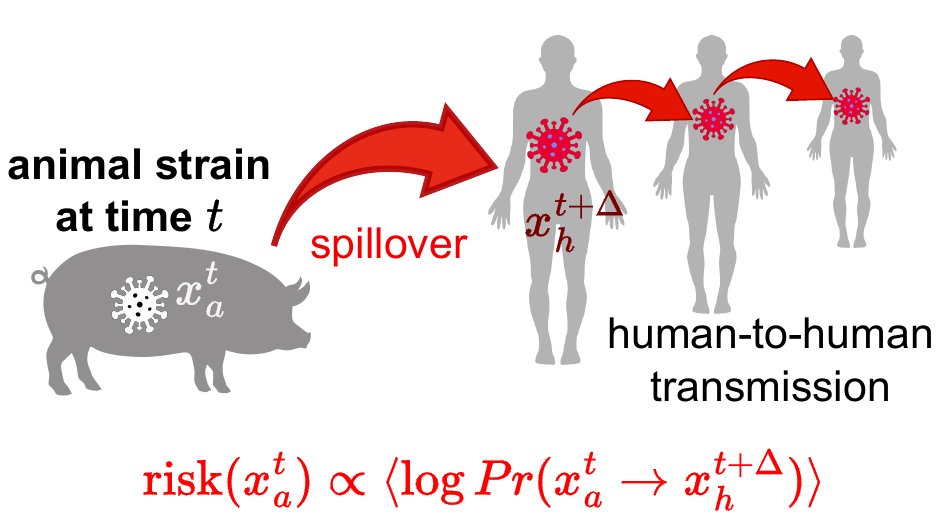
\includegraphics[width=2.5in]{Figures/External/f02}
  \vspace{-12pt}
  
  \captionN{Theoretical foundation of \bnd}\label{fig0}
\end{wrapfigure}
\infl, partly on account of its segmented genome and its wide prevalence in animal hosts, has the ability to incorporate genes from multiple strains and (re)emerge as novel human pathogens~\cite{reid2003origin,dos2016influenza}, thus harboring  a high pandemic potential. Strains spilling over into humans from animal reservoirs is thought to have triggered  mild to devastating pandemics  at least 4 times (1918 Spanish flu/H1N1, 1957 Asian flu/H2N2, 1968 Hong Kong flu/H3N2, 2009 swine flu/H1N1) in the past century~\cite{shao2017evolution}. One  approach to mitigating such risk is to recognize  animal strains  that do not yet circulate in humans, but are likely to spill-over and quickly achieve human-to-human (HH) transmission capability. While global surveillance efforts collect  wild specimens from diverse hosts/locations annually, our  ability to reliably and scalably  risk-rank individual strains remains limited~\cite{wille2021accurately}. CDC's current solution to this problem is the Influenza Risk Assessment Tool (IRAT)~\cite{Influenz24:online}.  SMEs
  score strains based on  the number of  human infections, transmission in laboratory animals, receptor binding, population immunity, genomic analysis, antigenic relatedness, global prevalence,  pathogenesis, and  treatment options, which are averaged to obtain 2 scores (between 1 and 10) that  estimate 1) the emergence  risk and 2) the potential public health impact on sustained transmission. IRAT scores  depend on multiple experimental assays,  taking  weeks/months to compile for a single strain. With tens of   thousands of strains being collected annually, this results in  a scalability bottleneck.

Here we plan to develop a platform powered by novel pattern discovery  algorithms to automatically parse out emergent evolutionary constraints operating on \infl viruses in the wild, to provide a less-heuristic theory-backed scalable solution to emergence prediction. We plan to show   that this capability enables preempting  strains which are \textit{expected to be in future human circulation}, and  approximate IRAT scores of non-human strains without  experimental assays or SME scoring, in seconds as opposed to weeks or months. Our approach automatically takes into account the time-sensitive variations in selection pressures as the background strain circulation evolves, and will potentially be able to rank-order strains adaptively.

Additionally, we plan to validate our ability to predict future variations of viral proteins by showing that predicted variants of HA are functional, and maintain replicative fitness in cell cultures.   Thus, bringing together rigorous data-driven modeling, and validation via tools from reverse genetics we plan to deliver an actionable and deployable platform (the \bnd) that optimally exploits the current biosurvellance capacity,  \textit{identifying when and where an imminent  emergence event is likely, and if such novel strains are likely to achieve human-to-human transmission capability.}

  
%he proper folding and cell surface expressing of predicted HA variants by flow cytometry as well as evaluate the fitness of recombinant viruses in a 1:1 competition experiments with parental strain.

\subsubsection*{Hypotheses} %State concisely the new insights, paradigms, technologies, or
% applications that address one of the FY23 PRMRP Topic Areas and one of the
% associated FY23 PRMRP Strategic Goals.

{\bf \itshape FY23 PRMRP Portfolio Category: Infectious Diseases $\vert$ FY23 PRMRP Topic: proteomics $\vert$  FY23 PRMRP Strategic Goal: Epidemiology: Identify strategies for surveillance or develop modeling tools and/or biomarkers to predict outbreaks or epidemics}
Our key hypotheses are as follows:
\begin{enumerate} 
[label=$\square$, leftmargin=0pt,
labelindent=0em, topsep=0.1em, labelsep=*, itemsep=.5em,itemindent=1em]
\item 
1) Learning  cross-dependencies across point mutations in key proteins, $e.g.$ those implicated in viral entry/exit (HA and NA) reveals  the underlying rules of organization of their primary structures to  forecast evolutionary trajectories, $i.e.$, predict future mutations and likelihood of jump events for animal strains. Importantly, while individual  sequences do  not encode enough information to predict its future mutations, discovering patterns from large sequence databases make such forecasts possible.
\item  
2) Current  bio-surveillance  produces sufficient data for meaningful pattern discovery, and  inferred  patterns of change can be assembled into an early warning system for pandemic threats, thus serving a similar function to the strategic goal of NORAD in the context of defending against geospatial pandemic threats, as opposed to protecting US airspace from adversarial intrusion.
\end{enumerate}
\subsubsection*{Specific Aims} We have three key aims described below: % – Specific Aims: Concisely explain the project’s specific aims and the objective(s) to
% be reached. These aims should agree with the primary aims and associated tasks
% described in the Statement of Work (SOW). If the proposed work is part of a larger
% study, present only aims that this DOD award would fund.
%Our specific aims are:
\begin{enumerate} 
[label=$\square$, leftmargin=0pt,
labelindent=0em, topsep=0.1em, labelsep=*, itemsep=.5em,itemindent=1em]
%########################
\item \textbf{Aim 1: Formulate a novel metric of sequence similarity (\qdist) that reflects potential of spontaneous jump.} Devise a  biologically meaningful metric for comparing two genomic sequences, that scales with the probability of one sequence spontaneously replicating to give rise to the other in the wild, under a) realistic, b) time-dependent, and c) poorly understood selection pressures. Within this aim, we will deliver the implemented  algorithm  identifying the \qdist metric as function of sub-type, gene, region and time, which is demonstrably distinct from the classical edit distance. Since the \qdist  reflects the odds of one sequence mutating  to  another, it is a function of not just how many mutations the two sequences are apart (the edit distance), but also how  specific mutations  incrementally affect fitness, and how possibly non-colocated mutations have  emergent dependencies and compensatory epistatic effects. Without these explicit constraints, assessing a strain-specific jump-likelihood  is open to subjective guesswork (current state-of-art). Our aim here is to show that a  precise probabilistic calculation is theoretically possible and practically feasible, enabling an actionable framework for tracking evolutionary change. The major tasks within this aim are as follows:
  \begin{inparaenum} \item[\bf T1.1 (\enet Development)] consisting of  sub-tasks: (T1.1.1) Precisely formulate the \enet inference platform, that puts together ML algorithms capturing maximally predictive patterns of change and mutational dependencies, and (T1.1.2) provide uncertainty quantification for the inferred patterns. \item[\bf T1.2 (Sample-complexity Estimation)]  Investigate  sample complexity of \enet, $i.e.$, how much data is needed to reliably identify  patterns. \item[\bf T1.3 (Event Timeline Estimation)] comprising 2 subtasks: (T1.3.1) Map mutational change dynamics to ``wall-time'', to  forecast \textit{when} future variants will show up, and (T1.3.2)  validate timeline predictions using records of  past emergence events, by assessing the time-delay between \enet predictions observation of predicted mutations in historical strain populations.
    \end{inparaenum}
%########################
  \item \textbf{Aim 2: Validate \qdist as a similarity metric  that can identify biologically meaningful sequence variations.} We aim to show that the \qdist may be used to differentiate between random perturbations in the genome  (most of which would be deleterious, and not code for a viable protein), and perturbations that are biologically viable. This is a key distinguishing capability of the \enet platform, that can reliably identify possible future mutations, along with their precisely quantified likelihoods.  We will demonstrate that  perturbations predicted using this metric leads to viable and functional proteins. The major tasks within this aim are: \begin{inparaenum}
    \item[\bf T2.1 (Quantify asymmetric transition probabilities between strains)] Key subtasks are: (T2.1.1) Infer probabilistic movement direction between strains, delineating the asymmetry of jump likelihood across strains, and (T2.1.2) chart multi-hop probabilistic trajectories from observed strains.    \item[\bf T2.2 (Laboratory Experiments for assessing fitness of predicted variants in cell culture)] consisting of the following subtasks: (T2.2.1) Shortlist HA variants with maximal emergence
probability of H3N2 and H1N1 subtypes, (T2.2.2) Generate predicted HA variants using reverse genetics in
human lung epithelial cell line (A549) and primary human lung cells, and (T2.2.3) evaluate generated variants for replicative fitness. These experimental assays will aim to demonstrate that strains with  small \qdist from observed strains leads to viable variants, and that even small random perturbations causes a catastrophic fall in fitness.
    \end{inparaenum} 
%########################
  \item \textbf{Aim 3:  Develop  a working implementation of \bnd.} We aim to demonstrate a prototype of the \bnd platform for analyzing \infl strains at scale  for emergence and impact risk. Major tasks are : \begin{inparaenum} \item[\bf T3.1 (IRAT score replication)] Replicate the published IRAT scores, along with uncertainty quantification,  within seconds as a validation result. Key subtasks are: (T3.1.1) Investigate how each of the ten IRAT dimensions  map to our \enet based risk,   (T3.1.2) Evaluate if the IRAT scores would change if evaluated at different times, and (T3.1.3) incorporate  timeline estimation in BioNORAD prototype to predict time to emergence.
\item[T3.2 (\bnd Results for Current/Recent Surveillance Data)] which comprises the subtasks: (T3.2.1) analyze collected sequences at scale, by enumerating the risk profiles of all sequences collected recently within the last few years, and any new sequences that continue to be submitted to NCBI and GISAID. And (T3.2.2) set up an automated pipeline that pulls in sequence data of for new submissions, and publish a risk score automatically. We will collate this information in our pipeline to map the global risk, visualizing where and when an emergence event is likely, and for which strain/subtype/animal hosts.
    \end{inparaenum} 

  \end{enumerate}



\begin{figure}[t]  
  \begin{tikzpicture}
    \node[label={}] (A) at (0,0) {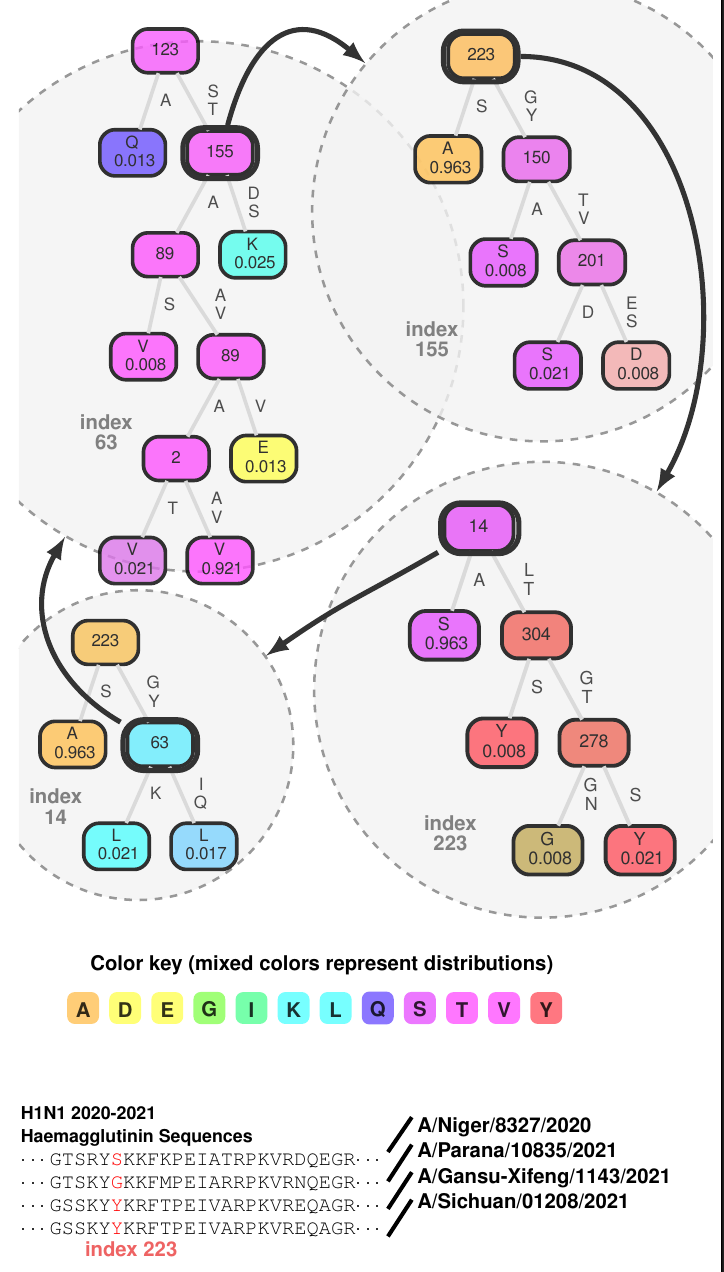
\includegraphics[width=2.65in]{Figures/External/f3}};
    \node[anchor=south west] (B) at (A.south east) {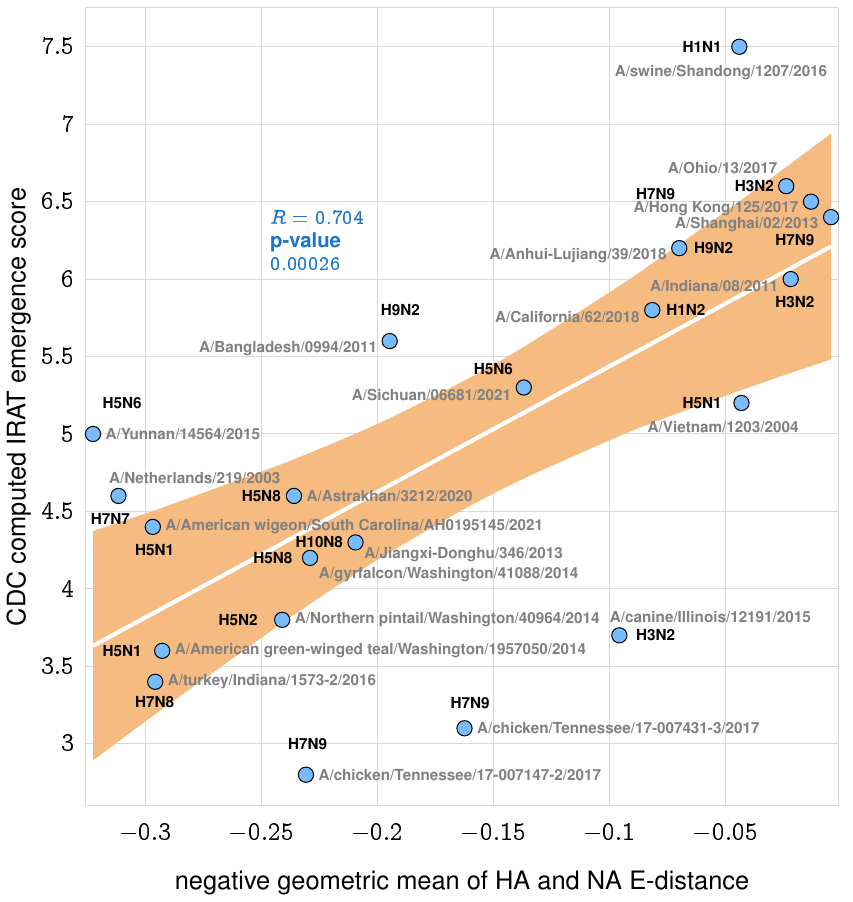
\includegraphics[width=4.6in]{Figures/External/f10}};
    \node[anchor=north west] (C) at ([yshift=-.1in]A.south west) {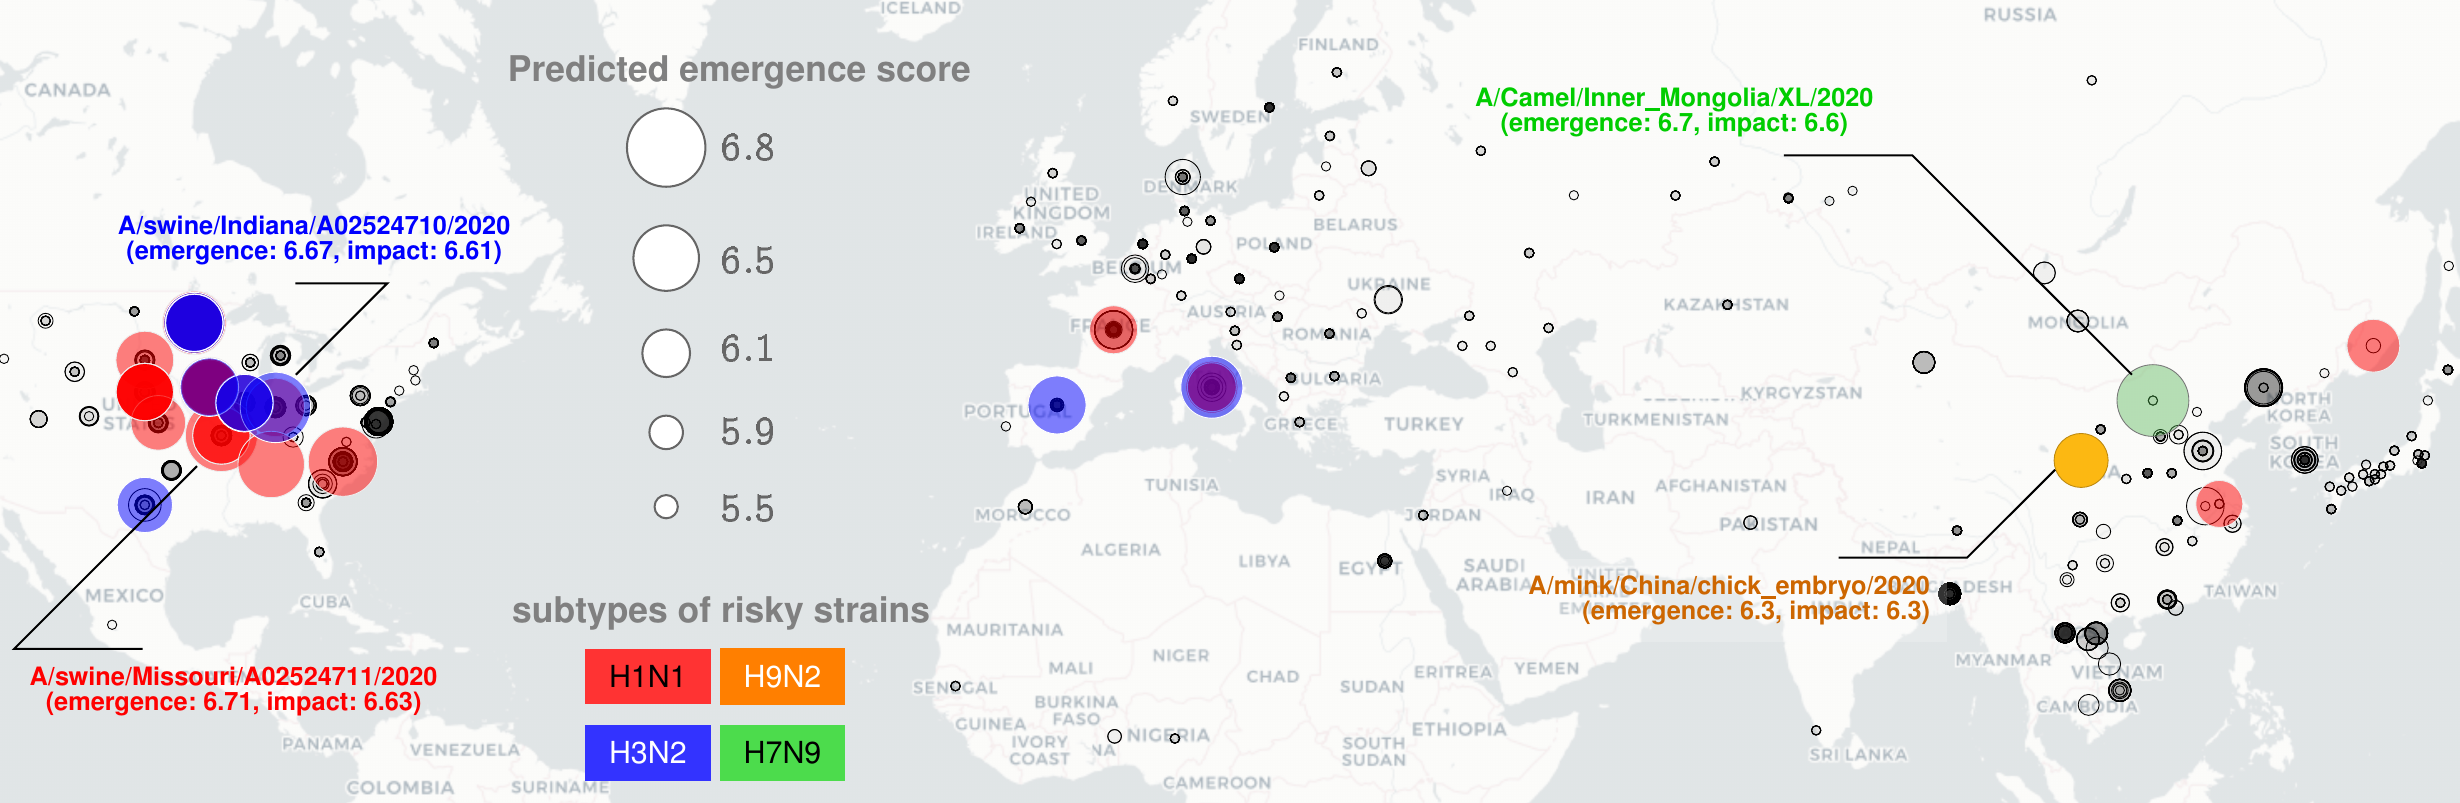
\includegraphics[width=\textwidth]{Figures/External/f11}};
\node[anchor=south west] (L1) at (A.north west) { \bf a. \enet structure};
\node[anchor=north west] (L2) at ([xshift=3in]L1.north west) { \bf b. IRAT score replication (with $\approx \times 10^6$ speedup)};
\node[anchor=south west] (L3) at ([yshift=-.15in]C.north west) { \bf  c. Preliminary \bnd implementation  current  potential emergence events};
\end{tikzpicture}
  \vspace{-15pt}

  \captionN{a, a fragment of an example \enet showing the emergent dependencies captured. b, IRAT replication in preliminary analysis with only HA sequence data, c, a preliminary \bnd implementation with sequences collected over 2021-2022, showing the emerging threat-centers, subtypes.}\label{fig1}

  \vspace{-20pt}

  
\end{figure}
\subsubsection*{Research Strategy and Feasibility} % – Research Strategy and Feasibility: Describe the experimental design, methods, and
% analyses, including appropriate controls, in sufficient detail for scientific evaluation.
% Address potential problem areas and present alternative methods or approaches. If
% cell lines or animals are to be used, justify why the proposed cell line(s) or animal
% model(s) were chosen. Describe how the proposed project will be completed within
% the proposed performance period.

Our approach aims  to reliably   estimate the non-heuristic numerical probability $Pr(x \rightarrow y)$ of a strain $x$ spontaneously giving rise to  $y$ in the wild, thus preempting  strains  expected to be in future circulation, and approximating IRAT scores of non-human strains without detailed  experimental assays or SME scoring. We plan to accomplish this by learning the complex cross-dependencies that constrain what a ``valid alteration'' of a AA sequence is, by first  analyzing  variations (point substitutions, indels) of   residue  sequences  of key proteins implicated  in cellular entry/exit~\cite{gamblin2010influenza,shao2017evolution}, namely HA and NA, and then expanding the analysis to the complete viral genome. By representing these constraints within a predictive framework -- the \enet (Enet) -- we will  estimate the  odds of a specific mutation to arise in future, and consequently the probability of a specific strain spontaneously  evolving into another (Fig.~\ref{fig0}). For such explicit calculations we must first infer the variation of mutational probabilities and  potential residue replacements from one positional index to the next along the AA sequence. The many well-known classical  DNA  substitution models~\cite{posada1998modeltest} or  phylogeny inference tools  assuming constant species-wise mutational characteristics,  are not applicable here. Similarly, newer algorithms such  as FluLeap~\cite{eng2014predicting}  which identifies host tropism and  species-level jump-risk~\cite{grange2021ranking} do not allow for strain-specific assessment.

The dependencies we expect to uncover are shaped by  a  functional necessity of conserving replicative  fitness. Strains must be sufficiently common  to be recorded in surveillance, implying that the sequences from public databases that we train  with have  high  fitness. Lacking kinetic proofreading, \infl integrates  faulty nucleotides   at a relatively high rate ($10^{-3}-10^{-4}$) during  replication~\cite{ahlquist2002rna,chen2006avian}. However, few variations are actually viable, leading to emergent dependencies between such mutations. Furthermore, these fitness constraints are  time-varying. The background strain distribution, and selection pressure from the evolution of cytotoxic T lymphocyte  epitopes~\cite{woolthuis2016long,fan2012role,van2016differential,berkhoff2007assessment,van2012evasion} in humans can change quickly. Our preliminary studies~\cite{chattopadhyay2022emergenet} suggest that we now have enough number of curated sequences in public databases to learn models that    automatically factor in the evolving host immunity, and the current background environment.  

Structurally, our model structure (an \enet) comprises an interdependent collection of  local predictors, each aiming to predict the  residue at a particular index  using as features  the residues   at other  indices  (Fig.~\ref{fig1}a). These individual predictors are implemented as conditional inference trees~\cite{Hothorn06unbiasedrecursive}, in which  nodal splits  occur with  a minimum pre-specified significance in differentiating the  downstream child nodes. The set of residues acting as features in each such predictor is automatically identified, $e.g.$, in the fragment of the  H1N1 HA \enet (2020-2021, Fig~\ref{fig1}a), the predictor for residue 63 is dependent on   residue  155, and the predictor for  155 is dependent on  223, the predictor for  223 is dependent on  14, and the residue at  14 is again dependent on  63, revealing a cyclic dependency. The complete \enet harbors a vast number of such  relationships, and each internal node of a tree may be  ``expanded'' to its own tree (since each index is ``explained'' by residues in other indices, which in turn have their own predictors). Owing to this recursive expansion,  a complete \enet  captures the intricate rules guiding evolutionary change as evidenced by our preliminary validations. Our research strategy comprises the following sequential steps:

\textit{(Step 1: Data and \enet Models)} We will collect AA sequences for the key genes of all available strains from NCBI and GISAID databases, and construct \enet{s} for each year,  each gene and each chosen geographical region. Different spatial and temporal resolutions will be considered in the course of the project, and we will consider all 8 genes in the \infl genome: PB2, PB1, PA, HA, NP, NA, M and NS. With about two decades worth of data comprising nearly $>380,000$ strains in NCBI and GISAID combined, when constructing models for each year, and the two hemispheres at a minimum, and the two subtypes H1N1 and H3N2, we end up with  $ 8 \times 20 \times 2 \times 2 = 640$ \enet models. With new emerging subtypes, the number of inferred models will be higher, and these models together capture the totality of observable statistically significant patterns constraining \infl evolution. 

\textit{(Step 2: \qdist metric calculation)} Each  \enet induces  an intrinsic distance metric (\qdist) between strains, collected at the time and space associated with the model, defined as the square-root of JS  divergence~\cite{cover} of the conditional residue distributions, averaged over the sequence. Unlike the classical approach of measuring the number of edits between sequences, the \qdist is informed by the \enet-inferred  dependencies, and adapts to the specific subtype, allele frequencies, and environmental variations. By our recent theoretical result~\cite{chattopadhyay2022emergenet},  \qdist  approximates the log-likelihood of spontaneous change $i.e.$ $\log Pr(x \rightarrow y )$, and despite general correlation between \qdist and edit-distance, the \qdist between fixed strains can change if only the background environment changes. 

\textit{(Step 3: Validation)} We aim to validate the predictive ability of the \enet framework in two ways: a) predict dominant strains in seasonal epidemics and compare against historical WHO vaccine recommendations in how well we can preempt the actual circulation in future seasons in the two hemispheres, and b) carry out  experimental assays in cell cultures to demonstrate that a perturbed strain is functional if the \qdist between the original and perturbed strain is small. 

\textit{Seasonal strain-forecast validation.} WHO  recommendations for the flu shot  is  formulated about 6-7 months in advance based on global circulation~\cite{agor2018models}. 
In  preliminary studies, our \enet-informed forecasts using only the HA gene outperform  WHO/CDC recommended flu vaccine compositions consistently over the past two decades, for both H1N1 and H3N2 subtypes, individually in the two hemispheres (which have distinct recommendations~\cite{boni2008vaccination}). For H1N1 HA, the \enet  recommendation outperforms  WHO  by $52.07\%$ on average over the last two decades, and $59.83\%$ on average in the last decade, and by $65.79\%$ in the period 2015-2019 (5 years pre-\cov). For H3N2 HA, the \enet  recommendation outperforms  WHO  by $42.39\%$ on average over the last two decades, and $35.00\%$ on average in the last decade, and by $41.85\%$ in the period 2015-2019. Despite limiting ourselves to only genotypic  information, our approach  distills  emergent  fitness-preserving constraints   that outperform or match reported DMS-augmented strategies~\cite{huddleston2020integrating,chattopadhyay2022emergenet}.

\textit{Assessment of fitness potential emerging zoonotic IAV variants in  cell culture.} Potential HA variants predicted by the \enet models will be generated using the reverse genetics system and evaluated for fitness against parental strains. Briefly, HA segments with potential mutations will be obtained through synthetic gene synthesis. We will assess the relative cell surface expression of parental HA and variants by flow cytometry and western
blotting. Next, we will generate recombinant viruses carrying mutant HA using an established reverse genetics system~\cite{pmid35926068,pmid34473799,pmid33970958,pmid32075925,pmid29899269,pmid28282445,pmid23686828,pmid20534532,pmid20126449} by the Manicassamy lab at UIowa, and validate the recombinant viruses by performing NGS sequencing. To assess the replication fitness of recombinant viruses, we will perform single cycle and multicycle replication assays human lung epithelial cell line (A549) and primary human lung cells~\cite{pmid23720581} (sourced from third-party vendors). In addition, we will assess the fitness of individual mutants by fitness competition assay with parental virus (1:1) and determine the relative ratio
by high resolution melting (HRM) analysis~\cite{ganti2021rab11a,wittwer2003high,marshall2013influenza} . These studies will help us determine the accuracy of \enet framework in predicting pandemic potential variants with enhanced fitness.  \textit{Choice of Cell-lines:} A549 cells and primary human lung cells are frequently used in  IAV experiments  due to their relevance to human infection, susceptibility to IAV, reproducibility, ease of cultivation, and compatibility with various molecular and cellular techniques~\cite{matrosovich1997avian}. These cells, derived from human lung carcinoma and lung tissue respectively, serve as appropriate models for studying IAV  pathogenesis, and host interactions, as they express key host factors~\cite{shinya2006influenza,chan2010tropism}, and are compatible with molecular and cellular techniques~\cite{neumann1999generation}. Dr. Manicassamy has $>15$ years of experience in working with human and zoonotic influenza viruses, and safely handling various human pathogens under enhanced BSL2 and BSL3 conditions.

\textit{(Step 4: \bnd Development)} Determining the numerical odds of a spontaneous jump $ Pr(x \rightarrow y)$  allows us to frame the problem of forecasting  dominant strain(s), and that of estimating the  pandemic potential of an animal strain as  mathematical propositions (albeit with some simplifying assumptions), with  approximate solutions (Fig.~\ref{fig0}). We will demonstrate that a pandemic risk score of a novel strain may be estimated by the probability of it giving rise to a well-adapted human strain. 
Our preliminary results~\cite{chattopadhyay2022emergenet} enable our ability to estimate the pandemic potential of novel animal strains, via a  time-varying \erisk score $\rho_t(x)$ for a strain $x$ not yet found to circulate in human hosts. We show that: $
\rho_t(x) \triangleq -\frac{1}{\abs{H^t}} \sum_{y \in H^t} \theta^{[t]}(x,y)
$ scales as the average log-likelihood of $Pr(x \rightarrow y)$ where $y$ is any human strain of a similar subtype to $x$, and  $\theta^{[t]}$ is the \qdist informed by the \enet computed from recent human strains $H_t$ at time $t$ of the same subtype as $x$, observed over the past year. The structure of dependencies revealed by the \enet inference makes it possible to estimate $\rho_t(x)$ explicitly. In the course of the project we will expand this risk score analytics to estimate the time to emergence in addition to spatial localization of such risk.
 
\textit{Preliminary Validation of \bnd.} We constructed \enet models for HA and NA sequences using subtype-specific human strains, typically collected within the  year prior to the assessment date. For rare human sub-types (H1N2, H7N7), we considered all subtype-specific human strains collected up to the  assessment date  to infer our \enet. For subtypes with little or no recorded human strains  (H5N2, H5N6, H5N8, H7N8, H9N2, H10N8), we constructed the \enet using all human strains that match the HA subtype alone. This addresses the issue of ``unknown unknowns'': allowing  \enet to assess  threats posed by not-yet-human strains. We  compute the \erisk for both HA and NA sequences (using the above relationship),  finally reporting their geometric mean as our estimated risk. Considering IRAT emergence scores of $22$ strains published by the CDC, we found strong out-of-sample support  (correlation: $0.704$, pvalue $<0.00026$, Fig.~\ref{fig1}b). Importantly, each \erisk score  is  computable in approximately $6$ seconds as opposed to weeks/months, suggesting a \textit{six order of magnitude speedup}. In the proposed study we will expand our analyis to incorporate all 8 genes. We show a preliminary implementation of the \bnd in Fig.~\ref{fig1}c for all 6,066 strains retrieved in 2021/22, showing the localization of  near-term threat events.

\subsubsection*{Innovation} %Innovation: Describe how the proposed research is innovative, including how it will
%provide new insights, paradigms, technologies, or applications to the research field
%and/or patient care. Investigating the next logical step of an existing line of research
%or providing an incremental advance on published data is not considered innovative.

Reported approaches to ``predicting'' mutations assume various models of DNA or AA substitution~\cite{posada1998modeltest,goldberger2005genomic,huelsenbeck1997phylogeny,neher2014predicting,VanderMeer2010,Smith2009} ignoring the impact of  a varying background and selection pressures. Importantly, a  higher edit-similarity between strains do not imply a high likelihood of a jump.
Current surveillance paradigms, and studies on habitat encroachment, climate change, and other  ecological factors~\cite{rulli2017nexus,chua2002anthropogenic,childs2004zoonotic}  have not improved our ability to actionably quantify future  risk of emergence of a specific strain from a specific host at a specific place~\cite{fair2019viral}. Recent advances in predicting seasonal  strains~\cite{huddleston2020integrating} also do not generalize to predicting emergence events, especially for strains that do not yet circulate in humans. This project innovates and envisions a path to acquiring this transformative capability, which is currently well-beyond the state-of-art: the \enet algorithm is  the first of its kind to learn an appropriate biologically meaningful comparison metric from data, without assuming any model of DNA or AA substitution, or a genealogical tree a priori, enabling an actionable pandemic early warning system. However, the potential impact of this work is not limited to pandemic preparedness, and can foster a more nuanced understanding of how viruses evolve and adapt over time. This could lead to the development of new therapeutic strategies that specifically target the evolutionary pathways of viruses, potentially revolutionizing the treatment of viral infections.
\clearpage
\mbox{}
\clearpage
\mbox{}
\clearpage
\mbox{}
\clearpage
\mbox{}
\clearpage
\mbox{}
\clearpage
\mbox{}
\clearpage
\mbox{}
\clearpage
\mbox{}
\clearpage
\mbox{}
\clearpage
\mbox{}
\clearpage
\mbox{}
\clearpage
\mbox{}
\clearpage
\mbox{}
\clearpage
\mbox{}
\clearpage
\mbox{}
\clearpage
\mbox{}
 

\clearpage
\limitpages{4}
%\HDR 


 

\clearpage
\mbox{}
\clearpage
\mbox{}
\clearpage
\mbox{}
\clearpage
\mbox{}
\clearpage
\mbox{}
\clearpage
\mbox{}
\clearpage
\mbox{}
\clearpage
\mbox{}
\clearpage
\mbox{}
\clearpage
\mbox{}
\clearpage
\mbox{}
\clearpage
\mbox{}
\clearpage
\mbox{}
\clearpage
\mbox{}
\clearpage
\mbox{}
\clearpage
\mbox{}
 

\clearpage

\limitpages{35}


% \ganttset{group/.append style={orange},
% milestone/.append style={red},
% progress label node anchor/.append style={text=red}}
% \begin{figure}[!hb]
%   \centering
%   \begin{ganttchart}[%Specs
%     expand chart=.85\textwidth,
%      y unit title=0.5cm,
%      y unit chart=0.7cm,
%      vgrid,hgrid,
%      title height=1,
% %     title/.style={fill=none},
%      title label font=\bfseries\footnotesize,
%      bar/.style={fill=blue},
%      bar height=0.7,
% %   progress label text={},
%      group right shift=0,
%      group top shift=0.7,
%      group height=.3,
%      group peaks width={0.2},
%      inline]{1}{24}
%     %labels
%     \gantttitle{A two-years project}{24}\\  % title 1
%     \gantttitle[]{Year 1}{12}                 % title 2
%     \gantttitle[]{Year 2}{12} \\              
%     \gantttitle{Q1}{3}                      % title 3
%     \gantttitle{Q2}{3}
%     \gantttitle{Q3}{3}
%     \gantttitle{Q4}{3}
%     \gantttitle{Q1}{3}
%     \gantttitle{Q2}{3}
%     \gantttitle{Q3}{3} 
%     \gantttitle{Q4}{3}\\
%     % Setting group if any
%     \ganttgroup[inline=false]{UCM Data Acquisition}{1}{3}\\ 
%     \ganttmilestone[inline=false]{IRB Approval}{2} \\
%     \ganttgroup[inline=false]{SSC Biosample Acquisition}{1}{4}\\ 
%     \ganttbar[progress=50,inline=false]{Biosample sequencing}{4}{18}\\
%  \ganttbar[progress=75,inline=false]{UCM Data Analysis}{3}{12}\\
%     \ganttmilestone[inline=false]{UCM analysis complete}{12} \\
%     \ganttmilestone[inline=false]{Year 1 Report}{12} \\
%     \ganttbar[progress=100,inline=false]{Biosample sequencing}{4}{18}\\
%       \ganttmilestone[inline=false]{Biosample sequencing complete}{18} \\
%    \ganttbar[progress=75,inline=false]{FInal analysis}{12}{24}\\
%      \ganttbar[progress=100,inline=false]{FInal analysis}{12}{24}\\
%     \ganttmilestone[inline=false]{Final Report}{24} \\
%   \end{ganttchart}
%   \captionN{Timeline and milestones}\label{figtimeline}
% \end{figure}



\clearpage

\section*{List of Abbreviations, Acronyms, and Symbols}


\begin{table}[!ht]
  \centering 
  %\captionN{Abbreviations Used}
 % \vskip .5em
  \hspace{-10pt}
  \begin{tabular}{R{2.5in}||L{3.55in}}\hline
      \rowcolor{Tomato!50} BioNORAD  & Proposed early warning system for pandemic risk (this proposal) \\
  \rowcolor{lightgray!50} AA residue  & Amino Acid residue \\
  \rowcolor{lightgray} AI  & Artificial Intelligence \\
  \rowcolor{lightgray!50} CDC & Centre for Disease Control \\
  \rowcolor{lightgray} CIT  & Conditional Inference Trees \\
  \rowcolor{lightgray!50} DMS & Deep mutational scanning \\
  \rowcolor{lightgray} GISAID  & Global Initiative on Sharing All Influenza Data \\
  \rowcolor{lightgray!50} HA  & Hemaglutinnin \\
  \rowcolor{lightgray} IAV & \infl virus \\
  \rowcolor{lightgray!50} IRAT  & Influenza Risk Assessment Tool\\
  \rowcolor{lightgray} JS Divergence & Jensen-Shannon Divergence\\
  \rowcolor{lightgray!50} ML  & Machine Learning \\
  \rowcolor{lightgray} NA  & Neuraminidase \\
  \rowcolor{lightgray!50} NCBI  & National Center for Biotechnology Information \\
  \rowcolor{lightgray} NORAD & North American Air Defense\\
  \rowcolor{lightgray!50} RBD  & Receptor Binding Site \\
  \rowcolor{lightgray} SME  & Subject Matter Expert \\
  \rowcolor{lightgray!50} UChicago &  University of Chicago \\
  \rowcolor{lightgray} UIowa &  University of Iowa \\
  \rowcolor{lightgray!50} UQ & Uncertainty Quantification\\
  \rowcolor{lightgray} WHO  & World Health Organization \\
  \rowcolor{lightgray!50} \qdist & \enet similarity between sequences\\    
  \rowcolor{lightgray} FluLeap & ML algorithm that uses sequence data to classify influenza viruses as either avian or human \\
  \rowcolor{lightgray!50} PRMRP &  Peer Reviewed Medical Research Program \\
  \rowcolor{lightgray} BSL2 &  Bio-safety Level 2 \\
  \rowcolor{lightgray!50} BSL3 &  Bio-safety Level 3 \\
  \rowcolor{lightgray} $\theta(x,y)$ &  \qdist between strains $x,y$ \\
  \rowcolor{lightgray!50} $\theta^{[t]}(x,y)$ &  \qdist between strains $x,y$ calculated at time $t$ \\
  \rowcolor{lightgray} $H_t$ &  recent human strains $H_t$ at time $t$ of similar subtypes if available. If the specific sub-type is rare, we progressively widen the definition to all strains with similar target gene. \\
    \rowcolor{lightgray!50} $\rho_t(x)$ &  time-varying \erisk score for emergence risk of strain $x$ \\
      \rowcolor{lightgray} $Pr(x\rightarrow y)$ & Probability of strain $x$ spontaneously mutating to produce strain $y$ in the wild \\
   \rowcolor{lightgray!50} $x_a^t$ & animal strain observed at time $t$ \\
    \rowcolor{lightgray} $x_h^t$ & human strain observed at time $t$ \\
    \rowcolor{lightgray!50} H1N1, H3N2, H5N1, H5N2, H9N2, H5N8, H7N8, H5N6, H10N8& \infl strains\\
    \rowcolor{lightgray}&\\
\hline

  \end{tabular}
  \end{table}



\clearpage

\limitpages{8}

\section*{Data Management Plan}
% 2 page limit



\subsection{Introduction} 

This Data Management Plan outlines the procedures for managing, storing, and sharing data generated during the course of the project on the analysis of hundreds of thousands of genomic sequences of Influenza A of various subtypes from public repositories (NCBI and GISAID). The research products include models and software, as well as example programs demonstrating how to access and read these models and apply them to raw data. An online system will also be developed to pull in new sequences from public databases, compute emergent risk, and display the results publicly. Experimental validation will involve specific protocols, cell lines, and procedures, which can be shared in an appropriate manner.

\subsection{Data Types and Formats}

This project will involve the following types of data:

\begin{itemize}
  \item Genomic sequences of Influenza A subtypes
  \item Metadata, including sequence IDs and other relevant information
  \item Models and software for generating, inferring, and reading the models
  \item Example programs demonstrating model access and application to raw data
  \item Experimental validation data, including protocols, cell lines, and procedures
\end{itemize}

All data will be stored in open and widely used formats, such as FASTA for genomic sequences, JSON or CSV for metadata, and standard programming languages like Python for software and example programs.

\subsection{Data Acquisition and Processing}

Data will be acquired from public repositories, such as NCBI and GISAID, and processed using custom-built software tools. These tools will parse the raw data and metadata, analyze the genomic sequences, and generate models to assess emergent risk. Quality assurance and quality control measures will be in place during data collection, analysis, and processing to ensure the reliability of the results.

\subsection{Data Storage and Preservation}

Data, models, and software will be stored on secure servers with appropriate backup and version control systems. Genomic sequences and metadata will be deposited in public repositories like NCBI and GISAID, while models and other data will be deposited at Zenodo for long-term access with DOI identifiers. Example programs and software tools will be hosted on GitHub repositories, ensuring easy access and collaboration.

\subsection{Data Sharing}

Data sharing will be achieved through a combination of methods:

\begin{itemize}
  \item Metadata and sequence IDs will be shared publicly, while respecting any restrictions on the genomic sequences themselves
  \item Models, software, and example programs will be available on GitHub repositories, allowing for easy access, collaboration, and updates
  \item Tools developed during the project will be easily installed from code registries like PyPI
  \item Experimental validation data, including protocols, cell lines, and procedures, will be shared in an appropriate and secure manner, ensuring compliance with any legal or ethical requirements
  \item An online system will provide public access to emergent risk assessment based on new sequences from public databases
\end{itemize}

\subsection{Handling of Restricted Data}

In cases where genomic sequences cannot be shared publicly due to legal or ethical constraints, the project will ensure that the handling and sharing of such data is in compliance with relevant regulations and guidelines. Sequence IDs and metadata will be shared, allowing other researchers to request access to the restricted sequences through appropriate channels. The project will have provisions in place for using sequences that are not publicly posted if the researchers or laboratories who collected the sequences do not grant permission to share them publicly. In such cases, the project team will collaborate with the data owners to determine the most appropriate way to utilize and share the data, ensuring that all parties' interests are respected and protected.


\subsection{Monitoring Adherence to the Data Management Plan}

Adherence to the Data Management Plan will be monitored throughout the project by a dedicated postdoctoral researcher, who will dedicate 5\% of their time to this task. The postdoctoral researcher will work under the supervision of the Principal Investigator, ensuring that the Data Management Plan is properly executed and that all project members are aware of their data management responsibilities.

Monitoring will include periodic reviews of data storage, sharing, and preservation practices, as well as ensuring that data quality assurance and quality control measures are effectively implemented. Any deviations from the plan will be addressed promptly, and the plan will be updated as needed to accommodate new data types, formats, or sharing requirements.

\subsection{Preservation Timeframe}

Data preservation will be maintained for a minimum of 10 years following the completion of the project. This timeframe will ensure that the research products remain accessible and usable by the scientific community for future research and development.
\subsection{Costs and Administrative Burden}

The Data Management Plan takes into consideration the balance between the value of data preservation and other factors such as associated costs and administrative burden. Data storage, preservation, and sharing costs will be factored into the project budget. A total of 5\% of the project's effort will be allocated to data management, including the postdoctoral researcher's time and any other administrative tasks related to data management.

The justification for any decisions regarding data preservation and sharing will be provided in the plan. This approach ensures that the research products are appropriately managed and shared, while also taking into account the costs and administrative burden associated with data management.

\subsection{Periodic Review of the Data Management Plan}

The Data Management Plan will be reviewed every six months by the Principal Investigator (PI) and co-Principal Investigator (co-PI) to ensure that it remains up-to-date and relevant to the project's needs. During these reviews, the PI and co-PI will assess the current data management practices and identify any necessary updates or changes to the plan.

These periodic reviews will help ensure that the Data Management Plan continues to be effective in guiding the project's data management activities and that it evolves as needed to accommodate new data types, formats, or sharing requirements. Any updates to the plan will be communicated to all project members to ensure that everyone remains informed about the project's data management expectations and responsibilities.

\subsection{Compliance with DoD Instructions}

This Data Management Plan adheres to the guidelines set forth in Section 3.c. Enclosure 3 of the Department of Defense (DoD) Instructions 3200.12. By following these guidelines, the project ensures that all data management practices are in compliance with the requirements of the DoD and that the data generated during the project will be appropriately managed, stored, and shared.
\begin{figure}[t]
  \centering
\definecolor{barblue}{RGB}{91,155,213}
\definecolor{groupblue}{RGB}{0,0,128}
\bf
\begin{ganttchart}[
    hgrid,
    vgrid,
    x unit=0.5cm,
    y unit chart=0.8cm,
    time slot format=isodate,
    time slot unit=month,
    bar/.append style={fill=barblue},
    group/.append style={draw=groupblue, fill=groupblue}
  ]{2023-10-01}{2025-10-01} % updated project duration
  \gantttitlecalendar{year, month} \\
  \ganttgroup{Project Duration}{2023-10-01}{2025-10-01} \\ % updated project duration
  \ganttbar{Software Deposition 1}{2023-10-01}{2023-10-01} \\
  \ganttbar{Software Deposition 2}{2024-04-01}{2024-04-01} \\
  \ganttbar{Software Deposition 3}{2024-10-01}{2024-10-01} \\
  \ganttbar{Model/Data Submission 1}{2024-04-01}{2024-04-01} \\
  \ganttbar{Model/Data Submission 2}{2025-04-01}{2025-04-01} \\
  \ganttbar[bar/.append style={fill=yellow}]{Experimental Protocol Sub.}{2024-04-01}{2024-04-01} \\
  \ganttbar[]{Final Software Submission}{2025-04-01}{2025-04-01} \\
  \ganttbar[bar/.append style={fill=orange}]{Final Data/Models Submission}{2025-10-01}{2025-10-01} \\
  \ganttlink{elem1}{elem2}
  \ganttlink{elem2}{elem3}
  %\ganttlink{elem3}{elem4}
  \ganttlink{elem4}{elem5}
  %\ganttlink{elem4}{elem6}
  \ganttlink{elem3}{elem7}
  \ganttlink{elem5}{elem8}
\end{ganttchart}

\captionN{DMP checkpoints. Software is deposited at Github repositories. Models and data are submitted at Zenodo.}
\end{figure}

\clearpage

\limitpages{8}

\section*{Data Management Plan}
% 2 page limit

\subsection{Introduction} 

This Data Management Plan outlines the procedures for managing, storing, and sharing data generated during the course of the project on the analysis of hundreds of thousands of genomic sequences of Influenza A of various subtypes from public repositories (NCBI and GISAID). The research products include models and software, as well as example programs demonstrating how to access and read these models and apply them to raw data. An online system will also be developed to pull in new sequences from public databases, compute emergent risk, and display the results publicly. Experimental validation will involve specific protocols, cell lines, and procedures, which can be shared in an appropriate manner.

\subsection{Data Types and Formats}

This project will involve the following types of data:

\begin{itemize}
  \item Genomic sequences of Influenza A subtypes
  \item Metadata, including sequence IDs and other relevant information
  \item Models and software for generating, inferring, and reading the models
  \item Example programs demonstrating model access and application to raw data
  \item Experimental validation data, including protocols, cell lines, and procedures
\end{itemize}

All data will be stored in open and widely used formats, such as FASTA for genomic sequences, JSON or CSV for metadata, and standard programming languages like Python for software and example programs.

\subsection{Data Acquisition and Processing}

Data will be acquired from public repositories, such as NCBI and GISAID, and processed using custom-built software tools. These tools will parse the raw data and metadata, analyze the genomic sequences, and generate models to assess emergent risk. Quality assurance and quality control measures will be in place during data collection, analysis, and processing to ensure the reliability of the results.

\subsection{Data Storage and Preservation}

Data, models, and software will be stored on secure servers with appropriate backup and version control systems. Genomic sequences and metadata will be deposited in public repositories like NCBI and GISAID, while models and other data will be deposited at Zenodo for long-term access with DOI identifiers. Example programs and software tools will be hosted on GitHub repositories, ensuring easy access and collaboration.

\subsection{Data Sharing}

Data sharing will be achieved through a combination of methods:

\begin{itemize}
  \item Metadata and sequence IDs will be shared publicly, while respecting any restrictions on the genomic sequences themselves
  \item Models, software, and example programs will be available on GitHub repositories, allowing for easy access, collaboration, and updates
  \item Tools developed during the project will be easily installed from code registries like PyPI
  \item Experimental validation data, including protocols, cell lines, and procedures, will be shared in an appropriate and secure manner, ensuring compliance with any legal or ethical requirements
  \item An online system will provide public access to emergent risk assessment based on new sequences from public databases
\end{itemize}

\subsection{Preservation Timeframe}

Data preservation will be maintained for a minimum of 10 years following the completion of the project. This timeframe will ensure that the research products remain accessible and usable by the scientific community for future research and development.

\subsection{Costs and Administrative Burden}

The Data Management Plan takes into consideration the balance between the value of data preservation and other factors such as associated costs and administrative burden. Data storage, preservation, and sharing costs will be factored into the project budget. The justification for any decisions regarding data preservation and sharing will be provided in the plan.



\clearpage
\mbox{}
\clearpage
\mbox{}
\clearpage
\mbox{}
\clearpage
\mbox{}
\clearpage
\mbox{}
\clearpage
\mbox{}
\clearpage
\mbox{}
\clearpage
\mbox{}
\clearpage
\mbox{}
\clearpage
\mbox{}
\clearpage
\mbox{}
\clearpage
\mbox{}
\clearpage
\mbox{}
\clearpage
\mbox{}
\clearpage
\mbox{}
\clearpage
\mbox{}
 
\clearpage
\limitpages{23}

\section*{Technical Abstract}
% 1 page limit
Our project aligns with the FY23 PRMRP Portfolio Category: Infectious Diseases, FY23 PRMRP Topic: proteomics, and FY23 PRMRP Strategic Goal: Epidemiology: Identify strategies for surveillance or develop modeling tools and/or biomarkers to predict outbreaks or epidemics.


Influenza A viruses, with their segmented genome and high prevalence in animal hosts, can  recombine genes from animal strains and (re)emerge as novel human pathogens. Pandemics triggered by animal \infl  strains spilling over into humans have occurred multiple times in the past century. Mitigating such risk involves identifying animal strains that have high odds of spilling over into humans and rapidly achieving human-to-human  transmission capability. While global surveillance efforts collect wild specimens annually, our ability to reliably and scalably risk-rank individual strains according their pandemic potential remains limited.
CDC's current solution to this problem is the Influenza Risk Assessment Tool (IRAT), which is based on subject matter experts scoring  strains-of-concern  on ten different phenotypic aspects  related to transmission and  pathogenicity on the basis of  multiple experimental assays. Thus scoring each strain can take  weeks to months. With tens of   thousands of strains being collected annually, this presents  a scalability bottleneck.

Here we propose to develop the BioNORAD platform to proactively identify  the risks posed by emerging Influenza A strains with high pandemic potential, akin to the strategic function of NORAD in defending the North American airspace. Powered by novel pattern discovery algorithms, our proposed algorithms will automatically parse emergent evolutionary constraints on Influenza A viruses in the wild. This platform will provide a less-heuristic, theory-backed, experimentally validated,  scalable solution to emergence prediction,  preempting strains expected in future human circulation and approximating IRAT scores of non-human strains a million times faster (seconds as opposed to weeks/months) without experimental assays or SME scoring. %We hypothesize that  learning patterns of cross-dependencies across point mutations from current sequence databases reveals enough of the  underlying rules of organization of their primary structures to actionably forecast evolutionary trajectories.

Our central insight here is that to preempt strains expected to be in future circulation, we need to reliably estimate the non-heuristic numerical probability of a strain x spontaneously giving rise to strain y in the wild. To accomplish this, we aim to  learn the complex cross-dependencies that constrain what a ``valid alteration'' of an amino acid (AA) sequence looks like (random perturbations are expected to be large deleterious), by first analyzing variations of residue sequences of key proteins implicated in cellular entry/exit, namely HA and NA, and then expanding the analysis to the complete viral genome. Our core algorithm, the \enet, leverages the inferred cross-dependencies to estimate the odds of a specific mutation arising in the future, and consequently the probability of a specific strain spontaneously evolving into another.

We will  validate our ability to predict future mutations by showing that \enet predicted HA variants express correctly, are functional, and maintain fitness unlike random modifications, via demonstrating proper folding, cell surface expression of  variants by flow cytometry as well as evaluate the fitness of recombinant viruses in  1:1 competition experiments with the unperturbed parental strain.

Finally these models will be assembled into a integrated platform (the \bnd) that  shows global near-time pandemic threat events as they emerge (from observation of new animal strains, as they are uploaded to the platform), along with estimates of the threat severity and estimated time to emergence.

Current surveillance paradigms, while crucial for mapping disease ecosystems, fail to address the challenge that a  higher edit-similarity between strains does not not imply a high likelihood of  jump.  % Efforts at tracking and modeling ecological factors driving up the odds of zoonotic spill-over have not improved our ability to quantify future risk of emergence of a specific strain from a specific host.
Also, recent advances in predicting seasonal  strains do not generalize to predicting emergence events, especially strains that do not yet circulate in humans, underscoring the problem of unknown unknowns. This project innovates and envisions a path to acquiring this transformative capability well-beyond the state-of-art. % The Emergenet algorithm is the first of its kind to learn an appropriate biologically meaningful comparison metric from data, without assuming any model of DNA or AA substitution, or a genealogical tree a priori, enabling an actionable pandemic early warning system.

The BioNORAD platform is crucial to US national interest, particularly in the context of protecting DoD assets and personnel deployed in potentially high-risk centers of emergence. Additionally, the platform will enable preemptive action, such as the inoculation of animal reservoirs before the first human infection, potentially eliminating the pandemic before it has a chance to trigger. The investment in the BioNORAD platform is thus a strategic step towards ensuring the health and safety of military personnel and the success of the DoD's mission in a world where pandemic threats are a growing concern.  The platform's ability to automatically factor in the evolving host immunity and the current background environment sets it apart from current state-of-the-art methods, making it a vital asset in the fight against pandemic threats and safeguarding military personnel, assets, and global health security.

\clearpage

\section*{Lay Abstract}
% 1 page limit
Our project aligns with the FY23 PRMRP Portfolio Category: Infectious Diseases, FY23 PRMRP Topic: proteomics, and FY23 PRMRP Strategic Goal: Epidemiology: Identify strategies for surveillance or develop modeling tools and/or biomarkers to predict outbreaks or epidemics.

Influenza A viruses have the potential to cause devastating pandemics, and  ongoing surveillance efforts are insufficient to reliably identify and rank strains with high pandemic potential. The current solution to this problem, the Influenza Risk Assessment Tool (IRAT) by the CDC, is subjective and slow requiring multiple experimental assays,  and thus cannot keep up with the scale of current global biosurveillance efforts.

To address this challenge, we propose to develop the \bnd  platform to proactively identify the risks posed by emerging Influenza A strains with high pandemic potential. The platform will use novel pattern discovery algorithms to automatically parse evolutionary constraints operating on Influenza A viruses in the wild, and provide an experimentally validated scalable solution to emergence prediction.

The Emergenet algorithm, at the core of the BioNORAD platform, is the first of its kind to learn an adaptive  biologically meaningful comparison metric from data, enabling an actionable pandemic early warning system. By reliably estimating the  numerical probability of a strain giving rise to another strain in the wild, the platform can preempt strains expected to be in future circulation, and approximate IRAT scores of non-human strains without experimental assays or subject matter expert scoring.

We will validate this core algorithm by  demonstrating that \enet predicted variations of genes from strains observed in the wild express correctly on host cell surfaces,  are functional, and do not lose replicative fitness, and hence  present potential future variants.

Ultimately the inferred models will be used to power the  \bnd platform that can track global threats from potential near-time emergence events as new strains are uploaded to the platform, along with  estimates of the threat severity and estimated time to emergence.

This represents a transformative capability, addressing the problem of unknown unknowns in the field of emergence modeling: state of the art tools are severely limited in their ability to predict or track emergence of novel strains. This knowledge gap renders the current substantial bio-surveillance efforts largely ineffective for precise actionable prediction of emergence events. These surveillance paradigms, while crucial for mapping disease ecosystems, fail to address the challenge of higher edit-similarity between strains not implying a high likelihood of a jump. Ongoing efforts at tracking and modeling ecological factors driving up the odds of zoonotic spill-over, while expensive,  have not improved our ability to quantify future risk of emergence of a specific strain from a specific host. Recent reported advances in predicting seasonal epidemic strain distributions  do not generalize to predicting emergence events as well, especially for novel subtypes  that do not yet circulate in humans.

By automating the analysis of influenza strains, the BioNORAD platform has the potential to revolutionize our ability to prevent pandemics before they emerge. It is a transformative technology that is urgently needed in a world where pandemics are a growing concern. By providing early warning of emerging strains, the platform can help prevent widespread outbreaks and save lives.

Furthermore, the BioNORAD platform has the potential to enable more proactive vaccination efforts. By identifying animal reservoirs of emerging strains before they jump to humans, public health officials could vaccinate these animals and prevent the emergence of pandemic strains, saving countless lives.

The BioNORAD platform can play a crucial role in protecting DoD assets and personnel deployed in potentially high-risk centers of emergence, and may make prophylactic inoculation possible against future strains.  Thus, the investment in the BioNORAD platform is a strategic step towards ensuring the health and safety of military personnel and the success of the DoD’s mission in a world where pandemic threats are a growing concern. 

Our project is a collaborative effort between experts in computer science, biology, and epidemiology, and all tools, software and data generated will be shared in accordance with DoD mandates.  This interdisciplinary approach is essential for developing a platform that can effectively address the complex problem of predicting pandemic risk. By bringing together experts from different fields, the platform can take advantage of cutting-edge advances in machine learning, bioinformatics, and epidemiology.

\clearpage





\clearpage
\limitpages{13}

\section*{Statement of Work - 04/26/2023}
% 3 page limit
\vskip 1em
\begin{center}
\textbf{\small PROPOSED START DATE 10/01/2023}
\vskip .5em

\begin{tabular}{R{.5in} |L{2.5in} |R{.5in}|L{2.5in}}
\hline
  Site 1: & \mnp{2in}{\vspace{5pt}
            University of Chicago\\ 5801 S. Ellis Ave.\\ Chicago, IL 60637 \\ PI: Ishanu Chattopadhyay
  \vspace{5pt}}  & Site 2: & \mnp{2in}{\vspace{5pt} University of Iowa\\51 Newton Road\\
Iowa City, IA 52242 \\ Site PI: Balaji Manicassamy }
  \\\hline
\end{tabular}
\end{center}

\begin{center}
  \vskip 1em

  
\gdef\HCOL{Tomato!50}
\gdef\MCOL{Lavender!50}
\begin{tabular}{|L{4.75in}|C{.75in}|C{.5in}|C{.5in}|}\hline
\rowcolor{\HCOL}\bf Specific Aim 1:  Formulate  sequence similarity metric  \qdist& \bf Timeline (Months)  & \bf Site 1 & \bf Site 2 \\\hline
\rowcolor{lightgray} Major Task 1.1: \ \enet Development &  & & \\\hline
Subtask T1.1.1: Precisely formulate the \enet inference platform, that puts together ML algorithms capturing maximally predictive patterns of change and mutational dependencies  & 1-3 & \checkmark& \\\hline
Subtask T1.1.2: Provide uncertainty quantification for the inferred patterns represented in the \enet models & 2-6  & \checkmark& \\\hline
  \rowcolor{\MCOL} \bf  Milestones Achieved:  M1)~\enet software beta release M2)~Uncertainty quantification of inferred models  & & &\\\hline
 \rowcolor{lightgray} Major Task 1.2:  Sample-complexity  for \enet inference  & & & \\\hline
 \rowcolor{\MCOL} \bf  Milestones Achieved: M3)~Sample-complexity estimates complete & & &\\\hline
  \rowcolor{lightgray} Major Task 1.3: \  Event Timeline Estimation & & & \\\hline
Subtask T1.3.1: Map mutational change dynamics to ``wall-time'' to  forecast \textit{when} future variants will show up  & 3-9 &\checkmark & \\\hline
Subtask T1.3.2: Computationally validate timeline predictions using records of  past emergence events  & 9-12  &\checkmark & \\\hline   \rowcolor{\MCOL} \bf Milestones Achieved: M4)~Software update for timeline estimation released  & & & \\\hline
 
\end{tabular}
\end{center}


\begin{center}

\begin{tabular}{|L{4.75in}|C{.75in}|C{.5in}|C{.5in}|}\hline
\rowcolor{\HCOL}\bf Specific Aim 2: Validate \qdist as a similarity metric on  strain space identifying biologically valid sequence variations & \bf Timeline (Months)  & \bf Site 1 & \bf Site 2 \\\hline
\rowcolor{lightgray} Major Task 2.1: Quantify asymmetric transition probabilities between strains &   & & \\\hline
Subtask 2.1.1 Develop analytical framework to identify probabilistic movement direction between strains & 9-12 &\checkmark & \\\hline
Subtask 2.1.2 Develop analytics to chart multi-step probabilistic trajectories from observed strains & 12-15 & \checkmark& \\\hline
  \rowcolor{\MCOL} \bf  Milestones Achieved: M5)~Software update for future trajectory calculation& & & \\\hline
 \rowcolor{lightgray} Major Task 2: Assessment of fitness of  potential emerging zoonotic IAV variants in cell cultures& & & \\\hline
Subtask 2.2.1 Shortlist HA variants with maximal emergence probability of H3N2 and H1N1 subtypes &  6-9& \checkmark& \checkmark\\\hline
Subtask 2.2.2 Generate predicted HA variants using reverse genetics in human lung epithelial cell line (A549) and primary human lung cells  &  9-22& &\checkmark \\\hline
Subtask 2.2.3 Evaluate generated variants for replicative fitness & 15-24 & & \checkmark\\\hline
  \rowcolor{\MCOL} \bf  Milestones Achieved: M6) \enet experimental validation complete & & & \\\hline 
\end{tabular}
\end{center}



\begin{center}

\begin{tabular}{|L{4.75in}|C{.75in}|C{.5in}|C{.5in}|}\hline
\rowcolor{\HCOL}\bf Specific Aim 3: Develop  a working implementation of \bnd & \bf Timeline (Months)  & \bf Site 1 & \bf Site 2 \\\hline
\rowcolor{lightgray} Major Task 3.1 IRAT score replication &  & & \\\hline
Subtask T3.1.1 Investigate how each of the ten dimensions of IRAT comparison map to our \enet based risk& 12-18 &\checkmark & \\\hline
Subtask T3.1.2 Evaluate sensitivity of  IRAT scores  to risk-assessment timepoint&  15-18&\checkmark & \\\hline
Subtask T3.1.3 Incorporate event timeline estimation in \bnd prototype to predict time to emergence &  18-24&\checkmark & \\\hline
  \rowcolor{\MCOL} \bf  Milestones Achieved: M7)~IRAT score-based validation of \bnd prototype & & & \\\hline
 \rowcolor{lightgray} Major Task 2: Results for Current/Recent Surveillance Data & & & \\\hline
Subtask T3.2.1 Demonstrate we can analyze collected sequences at scale, by enumerating the risk profiles of all sequences collected recently within teh last few years& 18-24 &\checkmark & \\\hline
Subtask T3.2.2 Set up an automated pipeline that pulls in sequence data of for new submissions, and publish a risk score automatically& 18-24 &\checkmark & \\\hline
  \rowcolor{\MCOL} \bf  Milestones Achieved: M8)~Working version of \bnd platform demonstrated M9)~Final project report submitted&  & & \\\hline 
\end{tabular}
\end{center}

\section*{Deliverables}

\begin{enumerate} 
[label=$\square$, leftmargin=0pt,
labelindent=0em, topsep=0.1em, labelsep=*, itemsep=.5em,itemindent=1em]
\item \enet software
\item \bnd implementation
  \item Experimental protocols for fitness assessment of \enet predicted strains
\end{enumerate}


\section*{Timeline}
The project timeline, indicating various milestones and tasks is illustrated in Fig.~\ref{figgantt}


\ganttset{group/.append style={orange},
milestone/.append style={red},
progress label node anchor/.append style={text=red}}
\begin{figure}[!hb]
  \centering
  \begin{ganttchart}[%Specs
    expand chart=.85\textwidth,
     y unit title=0.5cm,
     y unit chart=0.7cm,
     vgrid,hgrid,
     title height=1,
%     title/.style={fill=none},
     title label font=\bfseries\footnotesize,
     bar/.style={fill=blue},
     bar height=0.7,
%   progress label text={},
     group right shift=0,
     group top shift=0.7,
     group height=.3,
     group peaks width={0.2},
     inline]{1}{24}
    %labels
    \gantttitle{A two-years project}{24}\\  % title 1
    \gantttitle[]{Year 1}{12}                 % title 2
    \gantttitle[]{Year 2}{12} \\              
    \gantttitle{Q1}{3}                      % title 3
    \gantttitle{Q2}{3}
    \gantttitle{Q3}{3}
    \gantttitle{Q4}{3}
    \gantttitle{Q1}{3}
    \gantttitle{Q2}{3}
    \gantttitle{Q3}{3} 
    \gantttitle{Q4}{3}\\
    % Setting group if any
    \ganttgroup[inline=false]{Sequence Data Acquisition Pipeline}{1}{24}\\ 
    \ganttgroup[inline=false]{T1.1.1}{1}{3}\\ 
    \ganttgroup[inline=false]{T1.1.2}{2}{6}\\ 
    \ganttmilestone[inline=false]{Software beta release}{3} \\
    \ganttmilestone[inline=false]{Uncertainty quantification of  models}{6} \\
    \ganttgroup[inline=false]{T1.2}{3}{6}\\ 
    \ganttmilestone[inline=false]{Sample complexity estimated}{6} \\
    \ganttgroup[inline=false]{T1.3.1}{3}{9}\\ 
    \ganttgroup[inline=false]{T1.3.2}{9}{12}\\ 
    \ganttmilestone[inline=false]{Software update timeline estimation}{12} \\
    \ganttgroup[inline=false]{T2.1.1}{9}{12}\\ 
    \ganttgroup[inline=false]{T2.1.2}{12}{15}\\ 
    \ganttmilestone[inline=false]{Software update trajectory calculation}{15} \\
    \ganttgroup[inline=false]{T2.2.1}{6}{9}\\ 
    \ganttgroup[inline=false]{T2.2.2}{9}{22}\\ 
    \ganttgroup[inline=false]{T2.2.3}{15}{24}\\ 
    \ganttmilestone[inline=false]{Experimental validation complete}{15} \\
    \ganttgroup[inline=false]{T3.1.1}{12}{18}\\ 
    \ganttgroup[inline=false]{T3.1.2}{15}{18}\\ 
    \ganttgroup[inline=false]{T3.1.3}{18}{24}\\ 
    \ganttmilestone[inline=false]{IRAT score replication}{15} \\
    \ganttgroup[inline=false]{T3.2.1}{18}{24}\\ 
    \ganttgroup[inline=false]{T3.2.2}{18}{24}\\ 
    \ganttmilestone[inline=false]{\bnd working prototype}{15} \\
    \ganttmilestone[inline=false]{Final Report}{24} 
  \end{ganttchart}
  \captionN{Gantt chart of project timeline}\label{figgantt}
\end{figure}













\clearpage
\mbox{}
\clearpage
\mbox{}
\clearpage
\mbox{}
\clearpage
\mbox{}
\clearpage
\mbox{}
\clearpage
\mbox{}
\clearpage
\mbox{}
\clearpage
\mbox{}
\clearpage
\mbox{}
\clearpage
\mbox{}
\clearpage
\mbox{}
\clearpage
\mbox{}
\clearpage
\mbox{}
\clearpage
\mbox{}
\clearpage
\mbox{}
\clearpage
\mbox{}
 

\clearpage
\limitpages{14}
\section*{Impact Statement}
% 1 page limit
% Explain why the proposed research project is important and relevant to the FY23 PRMRP
% Topic Area addressed. Describe the FY23 PRMRP Strategic Goal that is addressed in the
% proposed research. Outline the potential impact, either short-term or long-term, of the
% proposed research on the field of study and/or patient care. Describe how the research 
% DOD FY23 Peer Reviewed Medical Discovery Award 26
% has the potential to generate preliminary data that can be used as a foundation for future
% research projects.
\subsubsection*{Relevance to FY23 PRMRP Topic Area}
The proposed research project is highly relevant to the proteomics topic area, specifically as it applies to infectious diseases caused by zoonotic emergence. The \enet algorithm can distill the emergent rules of organization of key viral proteins, uncovering how proteins respond to dynamic fitness landscapes and adapt to new hosts while evading host immune defenses. These investigations can provide key insights into protein evolution and reveal novel patterns that can aid in the discovery of vaccines and prevent the emergence of new virus strains.
% \subsubsection*{Relevance to  FY23 PRMRP Topic Area}
% The proposed research project is highly relevant to proteomics, specifically as it applies to the area of infectious diseases caused by zoonotic emergence. While we know that arbitrary variations in genomic sequences are deleterious, and mutations that allow animal viruses to adapt to human hosts must preserve function, the exact mechanisms that drive this balance between genotypic variation while producing functional proteins is unclear. Our \enet algorithm can distill the emergent rules of organization of the key viral proteins, and lay the foundation to uncovering how such proteins can respond to dynamic fitness landscapes, and  can vary enough to evade host immune defenses while preserving function and  adapting to new hosts. Ability to carry out these investigations at scale has the potential to reveal key insights in protein evolution. 

% Influenza A viruses are a major concern due to their pandemic potential, with past pandemics being triggered by animal strains spilling over into humans. The proposed research project aims to develop a platform that can proactively identify the risks posed by emerging Influenza A strains with high pandemic potential, akin to the strategic function of NORAD in defending the North American airspace.

% The development of the BioNORAD platform would represent a major advance in our ability to predict pandemics caused by Influenza A viruses, and would have significant implications for public health, biosurveillance efforts, and national security. The ability to rapidly and accurately risk-rank individual strains would be transformative in terms of our preparedness for potential pandemics, allowing us to take preemptive action and potentially eliminate pandemics before they have a chance to take hold.
\subsubsection*{Relevance to FY23 PRMRP Strategic Goal}
The proposed research project addresses the strategic goal of epidemiology, with a focus on identifying strategies for surveillance or developing modeling tools and/or biomarkers to predict outbreaks or epidemics. The BioNORAD platform provides a theory-backed, experimentally validated, and scalable solution to emergence prediction, preempting strains expected in future human circulation and approximating Influenza Risk Assessment Tool (IRAT) scores of non-human strains without experimental assays or subject matter expert scoring% . This represents a significant improvement in our ability to predict pandemics caused by Influenza A viruses.
%
% \subsubsection*{Relevance to  FY23 PRMRP Strategic Goal}
%
% The proposed research project addresses the FY23 PRMRP strategic goal of epidemiology, specifically the goal of identifying strategies for surveillance or developing modeling tools and/or biomarkers to predict outbreaks or epidemics. The current solution for assessing the risk posed by Influenza A strains, the Influenza Risk Assessment Tool (IRAT), is based on subject matter experts scoring strains of concern based on ten different phenotypic aspects related to transmission and pathogenicity, and takes weeks to months to compile for a single strain. With tens of thousands of strains being collected annually, this results in a scalability bottleneck.
%
% The BioNORAD platform represents a major step forward in terms of our ability to predict pandemics caused by Influenza A viruses. The platform is based on novel pattern discovery algorithms that automatically parse emergent evolutionary constraints on Influenza A viruses in the wild. It provides a less-heuristic, theory-backed, experimentally validated,  scalable solution to emergence prediction,  preempting strains expected in future human circulation and approximating IRAT scores of non-human strains without experimental assays or SME scoring
a million times faster. As a comparison, while 22 strains have been scored by the IRAT since 2013, we can analyze and score the entire GISAID and NCBI database in under a week with a moderately powerful computing cluster. This represents a significant improvement in our ability to predict pandemics caused by Influenza A viruses.

\subsubsection*{Potential impact, either short-term or long-term on the field of study and/or patient care}
The potential impact of the proposed research on the field of study and patient care is immense. Currently, pandemic preparedness and response is reactive and slow, often leading to significant loss of life and economic damage. The ability to accurately predict the emergence of high-risk pandemic strains before they have the opportunity to trigger a pandemic would revolutionize our approach to pandemic preparedness and response,  allowing us to rapidly develop and produce vaccines tailored to the specific strain before the pandemic even begins, potentially saving countless lives.

Furthermore, by understanding the evolutionary constraints and cross-dependencies that give rise to high-risk strains, we can begin to develop targeted interventions to prevent these strains from emerging in the first place. This could involve inoculating animal reservoirs with vaccines tailored to these high-risk strains or developing targeted surveillance efforts  in animals before they have the opportunity to jump to humans.

The potential impact of this work is not limited to pandemic preparedness, and can foster a more nuanced understanding of how viruses evolve and adapt over time. This could lead to the development of new therapeutic strategies that specifically target the evolutionary pathways of viruses, potentially revolutionizing the treatment of viral infections. In addition, the development of the BioNORAD platform has implications beyond Influenza A viruses. The methods developed as part of this work can be applied to other viruses with pandemic potential, such as coronaviruses and other respiratory viruses.

Overall, the potential impact of this work is significant, both in the short-term and long-term. By developing a better understanding of the evolutionary forces that give rise to high-risk pandemic strains and by providing an early warning system to identify emerging strains before they have the opportunity to trigger a pandemic, we can revolutionize our approach to pandemic preparedness and response, making this research project a critical investment in the future of our society.

\subsubsection*{Potential to generate preliminary data that can be used as a foundation for future research projects}
The BioNORAD platform's ability to predict the emergence of novel Influenza A strains with high pandemic potential, as well as estimate their evolutionary trajectories, will generate a wealth of data that can be used as a foundation for future research projects. The knowledge and insights gained from this research will facilitate the development of more effective and efficient biosurveillance methods and tools, as well as the design of new therapeutics and vaccines that target specific viral strains. Furthermore, this work will provide a framework for future studies aimed at predicting the emergence of other infectious diseases with pandemic potential.

In addition, the Emergenet algorithm's ability to learn an appropriate biologically meaningful comparison metric from data, without assuming any model of DNA or AA substitution or a genealogical tree a priori, represents a significant advance in the field of machine learning. This has the potential to impact a wide range of research areas beyond infectious disease epidemiology, such as protein structure prediction and drug design. The proposed research will not only advance our understanding of Influenza A evolution and pandemic risk assessment but also contribute to the broader scientific community's knowledge of machine learning and artificial intelligence.


\clearpage

\limitpages{15}
\section*{Relevance to Military Health Statement}
The proposed research project is highly responsive to the healthcare needs of military service members, veterans, and beneficiaries, specifically in regards to pandemic preparedness and response. The emergence of new strains of influenza viruses with the potential to cause pandemics is a global threat with significant implications for the health and safety of military personnel. Here we briefly discuss the incidence and/or prevalence of influenza in the general population as well as in military service members, veterans, and beneficiaries, describe the population(s)/dataset(s) to  be used in the proposed research project, and provide a description of how the knowledge, information, products, technologies, or applications gained from the research could be implemented in a dual-use capacity to benefit both military and civilian populations.

\subsection*{Incidence and Prevalence of Influenza}

Influenza is a highly infectious respiratory illness caused by the influenza virus. It affects millions of people worldwide each year and is responsible for a significant number of hospitalizations and deaths. According to the Centers for Disease Control and Prevention (CDC), in the United States alone, the estimated number of influenza-associated illnesses ranges from 9 million to 45 million annually, resulting in between 140,000 and 810,000 hospitalizations and between 12,000 and 61,000 deaths in a typical flu season \cite{CDC2021}. Military service members, veterans, and beneficiaries are not immune to the effects of influenza, and the Department of Defense (DoD) reports that influenza-like illness is one of the top five reasons for medical encounters among service members \cite{DoD2020}. In addition, influenza can have a significant impact on military readiness, with outbreaks resulting in decreased personnel availability and decreased mission effectiveness \cite{Wells2005}.

\subsection*{Population and Dataset}
The proposed research project will utilize a combination of publicly available genetic sequence data and epidemiological data from influenza surveillance programs. Specifically, the Global Initiative on Sharing All Influenza Data (GISAID) and the National Center for Biotechnology Information (NCBI) databases will be used to collect genetic sequence data on influenza viruses collected from human and animal hosts. Epidemiological data will be obtained from the World Health Organization (WHO) and the Centers for Disease Control and Prevention (CDC), including information on the geographic distribution of influenza strains and the incidence and prevalence of disease.

The use of these datasets is highly appropriate for the proposed research project. The GISAID and NCBI databases contain a wealth of genetic sequence data on influenza viruses collected from around the world. These databases are regularly updated and publicly available, ensuring that the research can be replicated and extended by other researchers. Additionally, the epidemiological data obtained from WHO and CDC are widely recognized as authoritative sources of information on influenza surveillance and are used by public health agencies around the world to track the spread of influenza.

Accessing these datasets is feasible, as they are publicly available and regularly updated. The use of these datasets also enables the research to be conducted at scale, allowing for the identification of emerging strains and the analysis of their evolutionary trajectories in a timely and efficient manner.

\subsection*{Dual-Use Capacity}
% Dual-use capacity
The knowledge and technologies gained from this research could be implemented in a dual-use capacity to benefit both military and civilian populations. The ability to predict and preempt the emergence of pandemic strains of influenza viruses has significant implications for global public health and biosurveillance efforts. By developing the BioNORAD platform, we can not only protect military personnel but also contribute to global efforts to prevent and respond to emerging infectious diseases.

The knowledge gained from this research project could also be applied to other infectious diseases with pandemic potential, such as coronaviruses and other respiratory viruses. The methods and algorithms developed as part of this work can be applied to other viruses with pandemic potential, potentially improving our ability to predict and respond to future pandemics, enabling us to act quickly and decisively to prevent the spread of the virus and save lives.

In conclusion, the proposed research project is highly responsive to the health care needs of military Service Members, Veterans, and/or beneficiaries. Influenza viruses are a major threat to military personnel deployed overseas, and the ability to predict and preempt pandemic strains of influenza viruses has significant implications for the health and safety of military personnel. The use of publicly available datasets and the interdisciplinary collaboration involved in this research project make it a highly feasible and appropriate approach to the problem. Finally, the dual-use potential of the research has significant implications for global public health and biosurveillance efforts, making it a critical investment in the future of both military and civilian populations.




\clearpage
\limitpages{100}
\section*{Facilities, Existing Equipment, and Other Resources}
\textbf{The University of Chicago} is a private non-profit institution located on the ethnically-diverse South Side of Chicago that has been a center of advanced learning and research since its inception in 1892. The University of Chicago is comprised of four graduate Divisions (Biological Sciences, Physical Sciences, Social Sciences, and Humanities), six professional schools (Chicago Booth School of Business, Divinity School, Harris School of Public Policy Studies, Law School, Pritzker School of Medicine, and School of Social Service Administration), the Graham School of General Studies, and the undergraduate College. The University has a unique history of organizing around research questions that cross disciplines rather than operating within  disciplinary boundaries. The extent to which this strategy reflects University of Chicago is illustrated by its numerous interdisciplinary Committees, Centers and Institutes (described below). The University of Chicago maintains its commitment to scholarship, teaching, and research through its more than 2100 faculty members and a student population of approximately 15,600 with nearly 2/3 engaged in advanced research and professional study. Through the years, 86 Nobel Laureates (8 are current faculty),  44 members of the National Academy of Sciences, 169 members of the American Academy of Arts and Sciences, and 14 recipients of the National Medal of Science have been associated with the University as students, teachers or research investigators. The University of Chicago is ranked among the world’s top universities by a number of criteria, including the amount of federal research funding received (despite a size much smaller than many of its academic peers). This spirit of discovery, innovation and public service provides a robust foundation for success.

% \textbf{The University of Chicago} is a private non-profit institution located on the ethnically-diverse South Side of Chicago that has been a center of advanced learning and research since its inception in 1892. The University of Chicago is comprised of four graduate Divisions (Biological Sciences, Physical Sciences, Social Sciences, and Humanities), six professional schools (Chicago Booth School of Business, Divinity School, Harris School of Public Policy Studies, Law School, Pritzker School of Medicine, and School of Social Service Administration), the Graham School of General Studies, and the undergraduate College. The University has a unique history of organizing around research questions that cross disciplines rather than operating within  disciplinary boundaries. The extent to which this strategy reflects University of Chicago is illustrated by its numerous interdisciplinary Committees, Centers and Institutes (described below). The University of Chicago maintains its commitment to scholarship, teaching, and research through its more than 2100 faculty members and a student population of approximately 15,600 with nearly 2/3 engaged in advanced research and professional study. Through the years, 86 Nobel Laureates (8 are current faculty),  44 members of the National Academy of Sciences, 169 members of the American Academy of Arts and Sciences, and 14 recipients of the National Medal of Science have been associated with the University as students, teachers or research investigators. The University of Chicago is ranked among the world’s top universities by a number of criteria, including the amount of federal research funding received (despite a size much smaller than many of its academic peers). This spirit of discovery, innovation and public service provides a robust foundation for success.

\textbf{South Shore Senior Health Center (SSSC):} The SSSC is a 6800 sq. ft. university-owned geriatric facility ~5 miles south of DCAM, with doorstep free parking in the heart of Chicago’s South Side, specifically in the South Shore district. There are 13 patient exam rooms equipped with an examination bed, ophthalmoscope and otoscope, in addition to an on-site phlebotomist and capability for ECG. There is a large conference room for team meetings and support groups. The Memory Center team meets on Mondays at this site.

\textbf{Center for Care and Discovery:} Completed in 2013, the CCD is a ten-story adult hospital focused on cancer, advanced surgery, high  tech  imaging,  the  neurosciences  and  gastrointestinal  procedures. The building is 1,200,000 GSF with floor plates of 102,000 GSF. The CCD includes 240 private patient rooms, 28 operating rooms (21 initially); an imaging department with 3 CT’s, 2 MRI’s, 1 fluoroscopy room, 2 general radiology rooms, 7 interventional radiology rooms; and a gastroenterology procedures suite with 11 GI procedure rooms, 2 fluoroscopy rooms and 2 bronchoscopy rooms.  The CCD includes an inpatient kitchen, cafeteria, 7th floor sky lobby meeting rooms, ground floor retail space and clinical support services. Two floors are “shelled space” for future expansion of services. The building is centrally located between existing clinical facilities (DCAM, Comer) and new research facilities (KCBD, GCIS, Knapp). The facility is connected to both DCAM and Comer via above and below ground connections. There are procedure rooms, 2 fluoroscopy rooms and 2 bronchoscopy rooms. Neurology and neurosurgery inpatients as well as a Neuro- ICU are contiguously located on one floor of the CCD. 

% \textbf{Department of Neurology:} The Department of Neurology, chaired by Dr. Shyam Prabhakaran, is a nationally recognized leader in neuroscience research. The department consists of 28 primary faculty and 21staff members. The department has multiple funded investigators and over 3 million dollars in extramural research. Along with the university and the BSD, the Department of Neurology places primary emphasis on the training of the next generation of academic leaders in neurology with a special focus on the development of clinician scientists. There has been expansion of the residency from 18 to 21 (7 per year). The department with UCM has launched the Clinical Neurosciences Service Line in 2019, directed by Dr. Prabhakaran, to integrate clinical care in neurology and neurosurgery across the spectrum of neurologic disease including community health and prevention, hospital-based acute care, and post-acute rehabilitation and re-integration in the community. The Service Line partners with the hospital and university to bring together resources including bioinformatics, quality improvement, clinical trials and research, and tele-technologies to enhance patient experience and outcomes.

% \textbf{Office Space:} The Neurology offices are housed in the UCM campus and medical center. It has 3 available conference rooms, teleconference capabilities, video conferencing capabilities both informally via internet-available software, as well as formally with WebEx. Dr. Mastrianni and the Executive Administrator will have private offices, as will the Outreach Core leader, and nurse. The coordinator and other staff members have dedicated workspaces in the Neurology office suite. All offices include: phone, pager, computer, scanner, fax, high-speed internet access and administrative support. Standard software available includes: SPSS, EndNote, Microsoft Access, and Adobe Acrobat Professional. The PD’s 300 sq foot office is equipped with a locked door and ample file storage. The research staff members are also equipped with locking file storage. In addition, the suite is protected by key card restricted access.

% \textbf{Memory Center:} Roughly 650 new patients and 1500 return patients are evaluated each year at the Memory Center. This is expected to rise, as an additional Behavioral Neurologist is being recruited as of this writing. Recruitment of most subjects will come from the Memory Center clinics. Two clinic sites are utilized. 1) the Duchossois Center for Advanced Medicine (DCAM) on the University of Chicago Medicine campus, and; 2) the South Shore Senior Health Center (SSSC), a 6800 sq. ft. university-owned geriatric facility approximately 5 miles south of DCAM, with convenient doorstep parking in the heart of Chicago’s South Side. Within the SSSC, in addition to referrals from the general geriatricians, there are specialty clinics that act as a referral to the Memory Center, including the Successful Aging and Frailty Evaluation (SAFE). The catchment area for the SSSC includes a large segment of south Chicago and northwestern Indiana, which currently has limited access to geriatrics and dementia specialists. Roughly 80\% of patients with cognitive problems at the SSSC are African American. 
 \section*{Computational Facilities}


The principal investigators have access to extensive computational facilities available at the University of Chicago to carry out the tasks described.


\textbf{Access to Clinical Data for AI-enabled Analytics:} The ZeD lab (overseen by Professor Chattopadhyay) is housed within the Department of Medicine at the University of Chicago, and has access to the full range of high end computing resources offered by the University of Chicago. In addition, Prof. Chattppadyay's laboratory has access to the HIPAA compliant clinical data warehouse maintained by the Biological Sciences Division as detailed below:

\textbf{The Clinical Research Data Warehouse:} (CRDW) within the Biomedical Sciences Division of the University of Chicago is one of the deepest, richest, and most research-ready data repositories of its kind. Containing more than a decade of University of Chicago medical data, it seamlessly brings together multiple internal and external data sources to provide researchers with access to more than 12 million encounters for 2.3 million patients. The associated diagnoses, labs, medications, and procedures number in the tens of millions each. The CRDW is run on IBM Netezza Pure Data System for Analytics servers, a patented Asymmetric Massively Parallel Processing architecture designed to deliver exceptional query performance and modular scalability on highly complex mixed workloads.

In order to meet the acute need for data related to COVID-19, the CRDW team has constructed three data marts (de-identified, limited, and identified) to provide the most commonly requested data elements for this patient population. The initial instance of the COVID-19 data mart includes de-identified structured data on patient demographics, encounters, diagnoses, labs, medications, flow sheets, and procedures. Additional data will be added based on resource availability and urgency.

\textbf{Cohort Discovery Tool:} The purpose of this tool (SEE Cohorts) is to provide a secure web-based tool for the initial exploration of de-identified data. It allows researchers to search available data, build a cohort of patients, and view actual de-identified data within the interface. The data in SEE Cohorts is refreshed weekly.

\textbf{Research Computing Center:} The University of Chicago Research Computing Center (RCC) provides high-end research computing resources to researchers at the University of Chicago, which include high-performance computing and visualization resources; high-capacity storage and backup; software; high-speed networking; and hosted data sets. Resources are centrally managed by RCC staff who ensure the accessibility, reliability, and security of the compute and storage systems. A high-throughput network connects the Midway Compute Cluster to the UChicago campus network and the public internet through a number of high-bandwidth uplinks. To support data-driven research RCC hosts a number of large datasets to be accessed within the RCC compute environment.

RCC maintains three pools of servers for distributed high-performance computing. Ideal for tightly coupled parallel calculations, tightly-coupled nodes are linked by a fully non-blocking FDR-10 Infiniband interconnect. Loosely-coupled nodes are similar to the tightly-coupled nodes, but are connected with GigE rather than Infiniband and are best suited for high-throughput jobs. Finally,  shared memory nodes contain much larger main memories (up to 1 TB) and are ideal for memory-bound computations. The types of CPU architectures RCC maintains are tabulated in Table~\ref{tabcap}.

\begin{table}
  \centering
  
\captionN{University of Chicago Research Computing Center Capabilities Summary}\label{tabcap}
\setlength{\arrayrulewidth}{1pt}
\sffamily\fontsize{9}{9}\selectfont
\begin{tabular}{||C{.8in}|c|R{1.85in}|R{.5in}|c||}\hline
\rowcolor{SeaGreen1}Cluster	&Partition&	Compute cores (CPUs)&	Memory	&Other configuration details\\\hline
midway1	&westmere&	12 x Intel X5675 3.07 GHz&	24 GB	& \\\hline
 	&sandyb	&16 x Intel E5-2670 2.6GHz&	32 GB	& \\\hline
 &	bigmem&	16 x Intel E5-2670 2.6GHz&	256 GB	& \\\hline
 	& &	32 x Intel E7-8837 2.67GHz&	1 TB&	 \\\hline
 	&gpu&	16 x Intel E5-2670 2.6GHz&	32 GB&	2 x Nvidia M2090 or K20 GPU\\\hline
 &	 &	20 x Intel E5-2680v2 2.8GHz&	64 GB&	2 x Nvidia K40 GPU\\\hline
 &	mic&	16 x Intel E5-2670 2.6GHz&	32 GB&	2 x Intel Xeon Phi 5100 coprocessor\\\hline
 &	amd&	64 x AMD Opteron 6386 SE&	256 GB&	 \\\hline
 &	ivyb&	20 x Intel E5-2680v2 2.8GHz&	64 GB&	 \\\hline
midway2&	broadwl&	28 x Intel E5-2680v4 2.4GHz&	64 GB&	 \\\hline
 &	bigmem2&	28 x Intel E5-2680v4 @ 2.4 GHz&	512 GB	 &\\\hline
 	&gpu2&	28 x Intel E5-2680v4 @ 2.4 GHz&	64 GB&	4 x Nvidia K80 GPU\\\hline
\end{tabular}
\end{table}


RCC also maintains a number of specialty nodes: 
\begin{itemize}
\item \textit{\color{gray} Large shared memory nodes} - up to 1 TB of memory per node with either 16 or 32 Intel CPU cores. Midway is always expanding, but at time of writing RCC contains a total of 13,500 cores across 792 nodes, and 1.5 PB of storage.
\item  \textit{\color{gray}  Hadoop:} Originally developed at Google, Hadoop is a framework for large-scale data processing.   \item  \textit{\color{gray}  GPU Computing:} Scientific computing on graphics cards can unlock even greater amounts of parallelism from code. RCC GPU nodes each include two Nvidia Tesla-class accelerator cards and are integrated in the Infiniband network. RCC currently provides access to Fermi-generation M2090 GPU devices and Kepler-generation K20 and K40 devices.  \item  \textit{\color{gray}  Xeon Phi:} The Many Integrated-Core architecture (MIC) is Intel's newest approach to manycore computing. Researchers can experiment with these accelerators by using  MIC nodes, each of which have two Xeon Phi cards, and are integrated into the Infiniband network.
\end{itemize}

\textbf{Persistent and High-Capacity Storage.} Storage is accessible from all compute nodes on Midway1 and Midway2 as well as outside of the RCC compute environment through various mechanisms, such as mounting directories as network drives on your personal computer or accessing data as a Globus Online endpoint (at the time of this writing, Globus Online is supported on Midway1). RCC takes snapshots of all home directories (users' private storage space) at regular intervals so that if any data is lost or corrupted, it can easily be recovered. RCC maintains GPFS Filesystem Snapshots for quick and easy data recovery.  In the event of catastrophic storage failure, archival tape backups can be used to recover data from persistent storage locations on Midway. Automated snapshots of the home and project directories are available in case of accidental file deletion or other problems. Currently snapshots are available for these time periods: 1) 7 daily snapshots, 2) 4 weekly snapshots.

\textbf{Tape Backups.} Backups are performed on a nightly basis to a tape machine located in a different data center than the main storage system. These backups are meant to safeguard against events such as hardware failure or disasters that could result in the complete loss of RCC’s primary data center.


\textbf{Data Sharing.} All data in RCC's storage environment is accessible through a wide range of tools and protocols. Because RCC provides centralized infrastructure, all resources are accessible by multiple users simultaneously, which makes RCC’s storage system ideal for sharing data among your research group members. Additionally, data access and restriction levels can be put in place on an extremely granular level.

\textbf{Data Security \& Management.} The HIPAA compliant security of the Research Computing Center’s storage infrastructure, protected by two-factor authentication,  gives users peace of mind that their data is stored, managed, and protected by HPC professionals. Midway's file management system allows researchers to control access to their data. RCC has the ability to develop data access portals for different labs and groups.





%\clearpage

% The principal investigators have access to extensive computational and experimental  facilities available at the University of Chicago and the University of Iowa to carry out the proposed project.

% \subsubsection*{University of Chicago facilities, equipment, and other resources}

% \textbf{Argonne Leadership Computing Facility (ALCF).}

% In partnership with Rick Stevens and Argonne National Lab, we will also have access to Argonne’s suite of high-performance machines, including ThetaGPU with 28 NVIDIA DGX-3 state-of-the-art AI systems, Polaris, which will be installed in spring, 2021 with 1024 NVIDIA A100 GPUs able to support ~7,000 simultaneous training sessions at once for problems that need hyper parameter optimization or for exploring properties of models. Aurora will be installed Summer 2022 and will host 60,000 Intel PVC-XT, performing AI inference at something like 64x faster at over 100 EFs per second, able to train up to 480K models in parallel and some very large models, supporting training models as high as 100 trillion parameters. Human brains have on order 100 trillion synapses (1011 neurons and 1.8-3.2 x 1014 synapses) and so this machine is, in some sense, a brain scale computer, likely the fastest on the planet when installed, and by far the fastest devoted to AI. Finally, we will have access to the National AI Accelerator Assessment Testbed (N3AT) Facility, designed to assess the usefulness of novel hardware designs from dozens of startups for advancing key research problems in AI. These include computers from Cerebras, SambaNova, Graphcore, Groq and many others. These models have the demonstrative ability to training transformer models, famously large in parameters, much more efficiently than within standard computing arrays (see Data and Computation). We will use Globus (www.globus.org) as a platform for data management, which provides managed data transfer solutions for high-speed, reliable, secure file transfer and replication among any variety of storage systems, including on-premise file systems and object stores, desktops and laptops, and cloud storage.


% ALCF also houses a range of other 
% high performance computing capabilities spearheaded by its 
% 10-petaflop IBM Blue Gene/Q system, Mira. 
% Mira is comprised of 48 racks, with 1,024 nodes per rack; 768 terabytes of RAM; 35 PB of storage; and 384 I/O nodes. 

% ALCF also hosts large storage systems. Mira data systems consist of 384 I/O nodes
% that connect to 16 storage area networks (SANs) that control 8,960 disk drives with 
% a total capacity of 28.8 PB of raw storage and a maximum aggregate transfer 
% speed of 240 GB/s. 
% ALCF computing resources share two 10,000-slot libraries using LTO4 tape technology. 
% The LTO tape drives have built-in hardware compression with compression ratios typically 
% between 1.25:1 and 2:1, depending on the data, giving an effective capacity of 16-24 PB.
% Two parallel file systems---PVFS and GPFS---are used to access the storage. 

% ALCF also operates a Globus-based data management and sharing pilot service called Petrel. 
% Petrel provides 1PB of storage that can be used by Argonne researchers and users of Argonne facilities to store and 
% share data with collaborators without the need for local account management. 


% \textbf{Research Computing Center:} The University of Chicago Research Computing Center (RCC) provides high-end research computing resources to researchers at the University of Chicago, which include high-performance computing and visualization resources; high-capacity storage and backup; software; high-speed networking; and hosted data sets. Resources are centrally managed by RCC staff who ensure the accessibility, reliability, and security of the compute and storage systems. A high-throughput network connects the Midway Compute Cluster to the UChicago campus network and the public internet through a number of high-bandwidth uplinks. To support data-driven research RCC hosts a number of large datasets to be accessed within the RCC compute environment.

% \textbf{Compute Infrastructure.} RCC maintains three pools of servers for distributed high-performance computing. Ideal for tightly coupled parallel calculations, tightly-coupled nodes are linked by a fully non-blocking FDR-10 Infiniband interconnect. Loosely-coupled nodes are similar to the tightly-coupled nodes, but are connected with GigE rather than Infiniband and are best suited for high-throughput jobs. Finally,  shared memory nodes contain much larger main memories (up to 1 TB) and are ideal for memory-bound computations. The types of CPU architectures RCC maintains are tabulated in Table~\ref{tabcap}.

% \begin{table}[!ht]
% \captionN{University of Chicago Research Computing Center Capabilities Summary}\label{tabcap}
% \setlength{\arrayrulewidth}{1pt}
% \bf\sffamily\fontsize{9}{10}\selectfont
% \begin{tabular}{||C{.8in}|c|R{1.85in}|R{.5in}|c||}\hline
% \rowcolor{SeaGreen1}Cluster	&Partition&	Compute cores (CPUs)&	Memory	&Other configuration details\\\hline
% midway1	&westmere&	12 x Intel X5675 3.07 GHz&	24 GB	& \\\hline
%  	&sandyb	&16 x Intel E5-2670 2.6GHz&	32 GB	& \\\hline
%  &	bigmem&	16 x Intel E5-2670 2.6GHz&	256 GB	& \\\hline
%  	& &	32 x Intel E7-8837 2.67GHz&	1 TB&	 \\\hline
%  	&gpu&	16 x Intel E5-2670 2.6GHz&	32 GB&	2 x Nvidia M2090 or K20 GPU\\\hline
%  &	 &	20 x Intel E5-2680v2 2.8GHz&	64 GB&	2 x Nvidia K40 GPU\\\hline
%  &	mic&	16 x Intel E5-2670 2.6GHz&	32 GB&	2 x Intel Xeon Phi 5100 coprocessor\\\hline
%  &	amd&	64 x AMD Opteron 6386 SE&	256 GB&	 \\\hline
%  &	ivyb&	20 x Intel E5-2680v2 2.8GHz&	64 GB&	 \\\hline
% midway2&	broadwl&	28 x Intel E5-2680v4 2.4GHz&	64 GB&	 \\\hline
%  &	bigmem2&	28 x Intel E5-2680v4 @ 2.4 GHz&	512 GB	 &\\\hline
%  	&gpu2&	28 x Intel E5-2680v4 @ 2.4 GHz&	64 GB&	4 x Nvidia K80 GPU\\\hline
% \end{tabular}
% \end{table}


% RCC also maintains a number of specialty nodes: 
% \begin{itemize}
% \item \textit{\color{gray} Large shared memory nodes} - up to 1 TB of memory per node with either 16 or 32 Intel CPU cores. Midway is always expanding, but at time of writing RCC contains a total of 13,500 cores across 792 nodes, and 1.5 PB of storage.
% \item  \textit{\color{gray}  Hadoop:} Originally developed at Google, Hadoop is a framework for large-scale data processing.   \item  \textit{\color{gray}  GPU Computing:} Scientific computing on graphics cards can unlock even greater amounts of parallelism from code. RCC GPU nodes each include two Nvidia Tesla-class accelerator cards and are integrated in the Infiniband network. RCC currently provides access to Fermi-generation M2090 GPU devices and Kepler-generation K20 and K40 devices.  \item  \textit{\color{gray}  Xeon Phi:} The Many Integrated-Core architecture (MIC) is Intel's newest approach to manycore computing. Researchers can experiment with these accelerators by using  MIC nodes, each of which have two Xeon Phi cards, and are integrated into the Infiniband network.
% \end{itemize}

% \textbf{Persistent and High-Capacity Storage.} Storage is accessible from all compute nodes on Midway1 and Midway2 as well as outside of the RCC compute environment through various mechanisms, such as mounting directories as network drives on your personal computer or accessing data as a Globus Online endpoint (at the time of this writing, Globus Online is supported on Midway1). RCC takes snapshots of all home directories (users' private storage space) at regular intervals so that if any data is lost or corrupted, it can easily be recovered. RCC maintains GPFS Filesystem Snapshots for quick and easy data recovery.  In the event of catastrophic storage failure, archival tape backups can be used to recover data from persistent storage locations on Midway. Automated snapshots of the home and project directories are available in case of accidental file deletion or other problems. Currently snapshots are available for these time periods: 1) 7 daily snapshots, 2) 4 weekly snapshots.

% \textbf{Tape Backups.} Backups are performed on a nightly basis to a tape machine located in a different data center than the main storage system. These backups are meant to safeguard against events such as hardware failure or disasters that could result in the complete loss of RCC’s primary data center.


% \textbf{Data Sharing.} All data in RCC’s storage environment is accessible through a wide range of tools and protocols. Because RCC provides centralized infrastructure, all resources are accessible by multiple users simultaneously, which makes RCC’s storage system ideal for sharing data among your research group members. Additionally, data access and restriction levels can be put in place on an extremely granular level.

% \textbf{Data Security \& Management.} The security of the Research Computing Center’s storage infrastructure gives users peace of mind that their data is stored, managed, and protected by HPC professionals. Midway’s file management system allows researchers to control access to their data. RCC has the ability to develop data access portals for different labs and groups.




\textbf{The Institute for Molecular Engineering at the University of Chicago} house a vibrant research community of multidisciplinary scientists that regularly collaborates to make significant scientific contributions. UChicago also features several translational resources, such as the Human Tissue Research Center, and the Transgenic Animal Center. 



\textbf{The University of Chicago Comprehensive Cancer Center (UCCCC):} One of only two NCI-designated Comprehensive Cancer Centers in Illinois, the UCCCC has a reputation for excellence and innovation and a commitment to address cancer through clinical and basic science cancer research and training, clinical cancer care, and expertise in population research. UCCCC researchers have access to a comprehensive set of shared technologies with the University of Chicago Biological Sciences Division (BSD), including 13 Core facilities. The UCCCC offers a wealth of intellectual, technological, and financial resources to pursue a comprehensive, collaborative research program involving more than 215 renowned scientists and clinicians.

\textbf{Translational and collaborative research:} The University of Chicago's strong physical sciences division, including my home department of Chemistry, is located in direct proximity to the medical school and hospital system. Indeed, I chose to start my independent career here at UChicago specifically so that I could develop a group whose work could impact human health. I have now witnessed firsthand the benefits of this proximity and have developed several strategic collaborations with clinicians and clinical researchers to develop new technologies. The University devotes substantial resources to translational research, which provides a clear path to move from the bench to the clinic. This includes the University of Chicago Innovation Exchange (https://innovation.uchicago.edu), which provides seed money and expertise to translate basic science discoveries into commercial ventures and to foster collaborations between the basic science divisions, medical school, and national labs. Therefore, the University of Chicago is an exceptional location to pioneer paradigm-shifting biomedical technologies.

% \textbf{University of Chicago Core Facilities} The University of Chicago offers extensive access to cutting-edge research technologies and expertise needed for my work via a well-funded and expertly staffed set of core facilities:
% \begin{itemize}
% \item The Microscopy Core – Maintains an extensive array of microscopes that our group can access, including a variety of confocal and 2-photon fluorescence scopes. The primary microscope we currently use is a Nikon Confocal featuring multiple laser excitation sources, a 2-photon light source, an automated stage, and a heated chamber. This will be very useful for the time course, live cell imaging experiments associated with the proposed research when our group’s microscope is insufficient. 
% \item The Biophysics Core - Provides access and training to state-of-the-art biophysics equipment, such as a Biacore, Plate Readers, and a ProteOn XPR36 protein interaction array system.
% \item  Transgenic/ES Cell Technology Mouse Core Facility - Provides genetically manipulated mice through transgenic technology or embryonic stem (ES) cell manipulation. The facility provides a comprehensive set of technical services and a fully operational construction and gene targeting service.

% \end{itemize}
% \section{Research Computing Center (RCC) at University of Chicago}

% The Research Computing Center (RCC) at the University of Chicago provides a variety of high-performance computing (HPC) systems for researchers across the university. These systems are used for a wide range of applications, including scientific simulations, data analysis, and machine learning.

% \subsection{HPC Systems}

% The RCC's HPC systems are based on the latest technologies and are designed to provide researchers with the performance and scalability they need to conduct their research. The systems are also highly reliable and are available 24/7.

% The RCC's HPC systems are available to all researchers at the University of Chicago. To access the systems, researchers must create an account and submit a job request. The RCC staff will then review the job request and, if approved, will submit the job to the appropriate system.

% The RCC's HPC systems are a valuable resource for researchers at the University of Chicago. These systems provide researchers with the performance and scalability they need to conduct their research and to make new discoveries.

% \subsubsection{Midway2}

% Midway2 is the RCC's primary HPC system. It is a large-scale cluster that consists of over 2,000 nodes. Each node contains two 16-core Intel Xeon E5-2697 v4 processors and 64GB of memory. Midway2 is connected by a high-speed InfiniBand network.

% Midway2 is a powerful system that can be used for a wide range of applications. It is particularly well-suited for scientific simulations, data analysis, and machine learning.

% \begin{table}[h]
%     \centering
%     \begin{tabular}{|l|l|}
%         \hline
%         Processor & 2 x 16-core Intel Xeon E5-2697 v4\\
%         \hline
%         Memory & 64GB per node\\
%         \hline
%         Network & High-speed InfiniBand\\
%         \hline
%     \end{tabular}
%     \caption{Midway2 specifications}
% \end{table}

% \subsubsection{Midway3}

% Midway3 is the RCC's newest HPC system. It is a smaller-scale cluster that consists of 100 nodes. Each node contains two 12-core Intel Xeon E5-2683 v4 processors and 64GB of memory. Midway3 is connected by a high-speed InfiniBand network.

% Midway3 is a high-performance system that is designed for researchers who need a more powerful system than what is available on Midway2. It is particularly well-suited for scientific simulations and data analysis.

% \begin{table}[h]
%     \centering
%     \begin{tabular}{|l|l|}
%         \hline
%         Processor & 2 x 12-core Intel Xeon E5-2683 v4\\
%         \hline
%         Memory & 64GB per node\\
%         \hline
%         Network & High-speed InfiniBand\\
%         \hline
%     \end{tabular}
%     \caption{Midway3 specifications}
% \end{table}

% \subsubsection{Other Systems}

% In addition to Midway2 and Midway3, the RCC also provides access to a number of other HPC systems. These systems include:

% \begin{itemize}
%     \item Beagle3: A small cluster that is designed for teaching and research.
%     \item DaLI: A GPU-accelerated cluster that is designed for machine learning.
%     \item MidwaySSD
% \end{itemize}

\subsubsection*{University of Iowa, Facilities and Other Resources}

\textbf{Laboratory Space.} Dr. Manicassamy's Laboratory is housed in the Department of Microbiology \& Immunology on the second floor
of the Bowen Science Building (BSB; Core 400) at The University of Iowa. This state of the art facility is
comprised of 1,700 square feet of newly renovated laboratory space. In addition to the infrastructure available
in the Department of Microbiology \& Immunology, Dr. Manicassamy’s research is supported by excellent core
facilities at the University of Iowa, including Next Generation Sequencing, Bioinformatics Core, Flow
Cytometry, Central Microscopy Research Facility, Small Animal Imaging, DNA sequencing. Dr. Manicassamy
has full-time administrative support through the Department of Microbiology \& Immunology.


\textbf{Office Space.} Dr. Manicassamy has 200 square feet of separate office space adjunct to the laboratory in BSB. PC and Mac
computers, computational network, laser printers, color printers, and scanners are available. Manuscripts and
desktop publishing of papers can be prepared in several offices available to scientists working in BSB.


\textbf{Scientific Environment. } The University of Iowa has a highly collaborative research community with several leading Virologists and
Immunologists, including Drs. Stanley Perlman (Coronaviruses pathogenesis/host responses), Mark Stinski
(Herpes Virus), John Harty (T cell responses to Infection), Kevin Legge (dendritic cell-T cell responses to
Influenza virus), Steven Varga (Host responses to RSV), Gail Bishop (Viral Immunology), Wendy Maury
(Filovirus entry), Richard Roller (Molecular Herpes virology), Jack Stapleton (HIV/HCV pathogenesis), and
Hillel Haim (HIV evolution/pathogenesis). Weekly Microbiology seminar series, and the Virology and
Immunology journal clubs provide excellent opportunities for students and postdocs for scientific interactions.
In addition, research program in pulmonary biology provide an excellent scientific forum for discussion and
collaboration. The Levitt Center for Viral Pathogenesis provides funding for seminar speakers and student
travel and is another venue for interactions with research interests related to the project. Moreover, the
students and postdocs are supported by several NIH T32 training grants.


\textbf{Animal Care Unit (ACU)} at The University of Iowa is in full compliance with all NIH guidelines and regulations
pertaining to the care and use of experimental animals (PHS Assurance no. A3021-01). The ACU has enjoyed
accreditation from the American Association of Accreditation of Laboratory Animal Care since 1994. The ACU
maintains centralized animal housing facilities, which are staffed by highly trained individuals to provide
husbandry and research support services. In addition to providing daily animal care, all ordering and receipt of
animals, quarantine and health monitoring is performed by the ACU. The ACU also provides research support
services, such as anesthesia and surgical support, rodent breeding assistance, diagnostic laboratory services,
and investigator training. The ACU veterinarians are faculty members of The University of Iowa. They are
available to assist investigators and their staff with all aspects of their animal research activities.

\textbf{Biosafety Facility.} The select agent containment laboratories are housed on the 5 rd floor of the Carver Biomedical Research
Building (CBRB) and on the 4 th floor of the Medical Laboratories (ML) Building, University of Iowa, Iowa City,
IA. BSL3 facilities are CDC certified and is managed by Ms. Dana Reis (Director). Dr. Manicassamy has one
BSL3 suite with one class IIb biosafety cabinet and one Animal BSL3 suite available for work on highly pathogenic influenza viruses and coronaviruses.

\subsection*{Major Equipment in Dr. Manicassamy's laboratory:}



\begin{enumerate}
\item \textbf{Biosafety cabinets:} Sterile environment for handling infectious materials, safeguarding researcher and samples.
\item \textbf{Tissue culture incubators:} Optimal temperature, humidity, and gas conditions for cell and tissue growth.
\item \textbf{PCR machines and real-time PCR machines:} Amplify specific DNA sequences, monitor amplification process in real-time.
\item \textbf{Table top centrifuges:} Separate liquid sample components based on density.
\item \textbf{Microscopes:} Visualize microscopic organisms, cells, and minute structures.
\item \textbf{-80 freezers and -20 freezers:} Long-term storage and preservation of biological samples.
\item \textbf{Bacterial incubators:} Optimal conditions for bacterial growth and development.
\item \textbf{Bacterial shakers:} Facilitate aeration and mixing of bacterial cultures.
\item \textbf{Thermal cyclers:} Precise temperature control for DNA amplification and molecular biology applications.
\item \textbf{UV-Spectrophotometers:} Measure light absorbance, determine concentration and purity of biomolecules.
\item \textbf{Fluorescence microscope:} Visualize and analyze samples using fluorescence, study cellular structures and biomolecular interactions.
\item \textbf{Gel doc unit:} Capture and document images of DNA, RNA, and protein samples in gel electrophoresis experiments.
\end{enumerate}

\textbf{University of Iowa Department of Microbiology and Immunology Resources:}

\begin{enumerate}
\item \textbf{3 flow cytometers:} Measure and analyze physical and chemical properties of cells or particles in fluid.
\item \textbf{Fluorescence plate readers:} Measure fluorescence intensity in microplate format, high-throughput analysis of cellular and biochemical events.
\item \textbf{Zeiss inverted fluorescent and confocal microscopes:} High-resolution imaging of biological samples, visualize living cells and tissues.
\item \textbf{qRT-PCR thermocyclers:} Quantify RNA transcripts in real-time, provide insights into gene expression.
\item \textbf{Fuji CCD imaging system:} Capture high-resolution images of fluorescent and chemiluminescent samples, sensitive and accurate detection of biomolecules.
\item \textbf{High-speed and ultracentrifuges with varied rotors:} Rapid separation of samples based on size, shape, and density, accommodate various rotor types.
\item \textbf{Typhoon imaging system:} Detect, quantify, and analyze proteins, nucleic acids, and biomolecules in gels, membranes, and microplates.
\item \textbf{ELISA plate readers:} Measure absorbance of enzyme-linked immunosorbent assays (ELISA), quantify proteins, peptides, and hormones.
\item \textbf{TopCount:} High-throughput quantification of radioactivity in samples, study biochemical and cellular processes.
\item \textbf{LiCor imaging system:} Sensitive and accurate detection of fluorescent and chemiluminescent samples in various formats.
\item \textbf{Darkroom facilities:} Controlled processing of light-sensitive materials, such as photographic films and imaging plates.
\item \textbf{Cold and warm rooms:} Temperature-controlled spaces for storage and experiments requiring specific temperature conditions.
\end{enumerate}


\clearpage

\section*{Publications and/or Patents}

\subsection*{Patents}
\vskip 1em

\begin{enumerate} 
[label=$\square$, leftmargin=0pt,
labelindent=0em, topsep=0.1em, labelsep=*, itemsep=.5em,itemindent=1em]
\item Chattopadhyay, I. (2022). ``Methods and systems for genomic based prediction of virus mutation'' (Patent No. WO2022108965A1). World Intellectual Property Organization. URL: \url{https://patents.google.com/patent/WO2022108965A1}
\end{enumerate}

\textbf{Abstract:} 
A method includes receiving a first plurality of aligned genomic sequences of a virus from a database. The aligned genomic sequences have a first common background. The method includes calculating a Qnet for each genomic sequence of the first plurality of aligned genomic sequences. The Qnet for each sequence is calculated by calculating a conditional inference tree for each index of the aligned genomic sequences using other indices in the aligned genomic sequences as predictive features, and calculating predictors for indices that were used as predictive features when calculating the conditional inference tree for each index.

\vskip 1em



% \begin{table}[!ht]
%   \captionN{Pending Patent on Core Algorithm}\label{tabpatent}
%   \begin{tabular}{R{1.5in}L{5in}}
% Title&  METHOD OF CREATING ZERO-BURDEN DIGITAL BIOMARKERS FOR DISORDERS AND EXPLOITING CO-MORBIDITY PATTERNS TO DRIVE EARLY INTERVENTION \\
% Patent Application Type & International\\
% International Filing Date & 09/23/2020 \\
% International Application No.& PCT/US2020/052112 \\
% Publication Number &  WO/2021/061702 \\
% Applicant & The University of Chicago\\
% Priority Data &  62/904,220, 09/23/2019 US

%                             62/937,604, 11/19/2019 US \\
%     WIPO IP Portal Link & \url{https://patentscope.wipo.int/search/en/detail.jsf?docId=WO2021061702}\\
% IP Filing Plans & File non-provisional patent application in the United States and foreign jurisdictions by nationalization date 03/23/2022\\\hline
%   \end{tabular}
%   \end{table}


\subsection*{Relevant Publications}

\begin{enumerate} 
[label=$\square$, leftmargin=0pt,
labelindent=0em, topsep=0.1em, labelsep=*, itemsep=.5em,itemindent=1em]
\item Huang, Yi, and Ishanu Chattopadhyay. ``Universal risk phenotype of US counties for flu-like transmission to improve county-specific COVID-19 incidence forecasts.'' PLoS computational biology 17, no. 10 (2021): e1009363. DOI: \url{https://doi.org/10.1371/journal.pcbi.1009363}

\item Dhanoa, J., Manicassamy, B. and Chattopadhyay, I., 2018. ``Algorithmic Bio-surveillance For Precise Spatio-temporal Prediction of Zoonotic Emergence.'' arXiv preprint arXiv:1801.07807. Preprint DOI: \url{https://arxiv.org/abs/1801.07807} 

\item Chattopadhyay, Ishanu, Emre Kiciman, Joshua W. Elliott, Jeffrey L. Shaman, and Andrey Rzhetsky. ``Conjunction of factors triggering waves of seasonal influenza.'' Elife 7 (2018): e30756. DOI: \url{https://doi.org/10.7554/eLife.30756}

\item Li, Jin, Timmy Li, and Ishanu Chattopadhyay. ``Preparing For the Next Pandemic: Learning Wild Mutational Patterns At Scale For For Analyzing Sequence Divergence In Novel Pathogens.'' medRxiv (2020): 2020-07. Preprint DOI: \url{https://doi.org/10.1101/2020.07.17.20156364}

  \item Chattopadhyay, Ishanu, Kevin Wu, Jin Li, and Aaron Esser-Kahn. ``Emergenet: Fast Scalable Pandemic Risk Assessment of Influenza A Strains Circulating In Non-human Hosts.'' (2022). Preprint DOI: \url{https://doi.org/10.21203/rs.3.rs-2336091/v1}

\end{enumerate}

\clearpage

%\section*{Letters of Organizational Support}
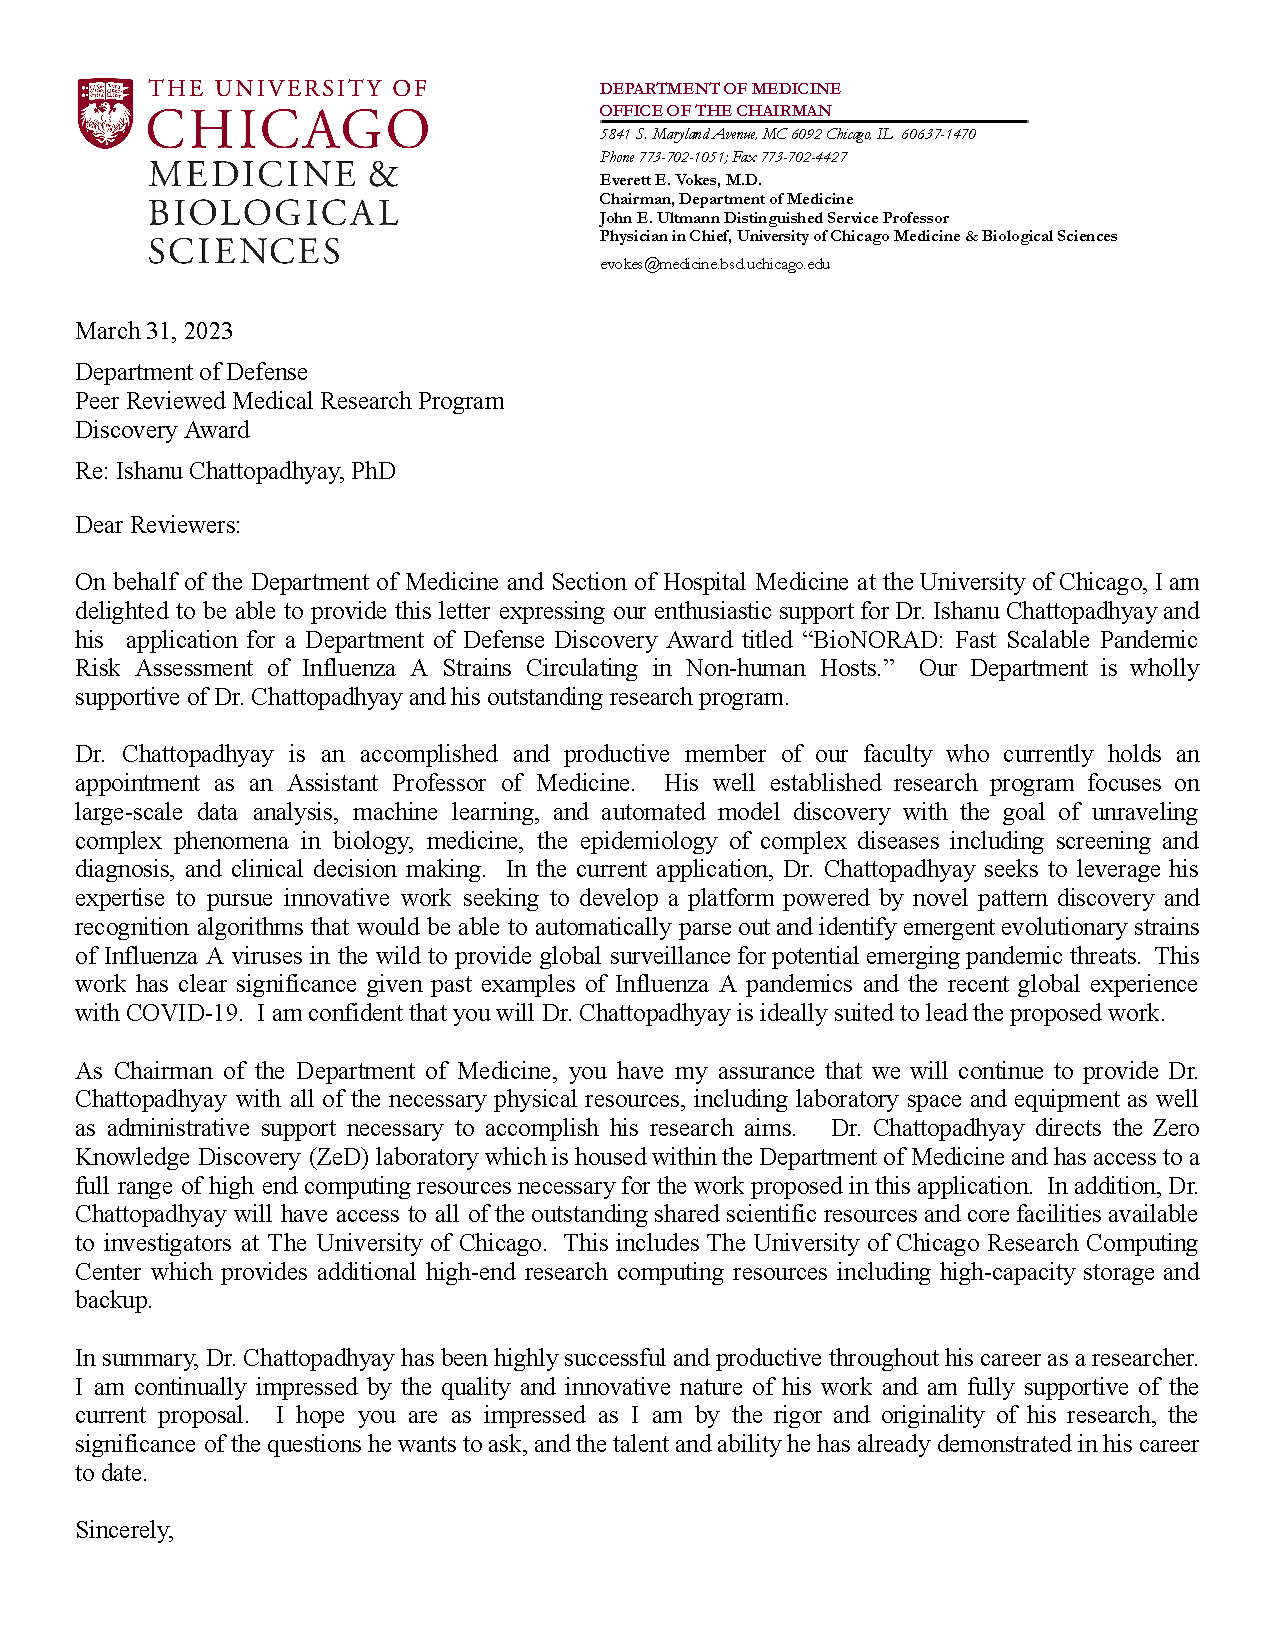
\includepdf[pages=-]{Figures/LOS-chair.pdf}

\clearpage

% \section*{Letters of Collaboration}
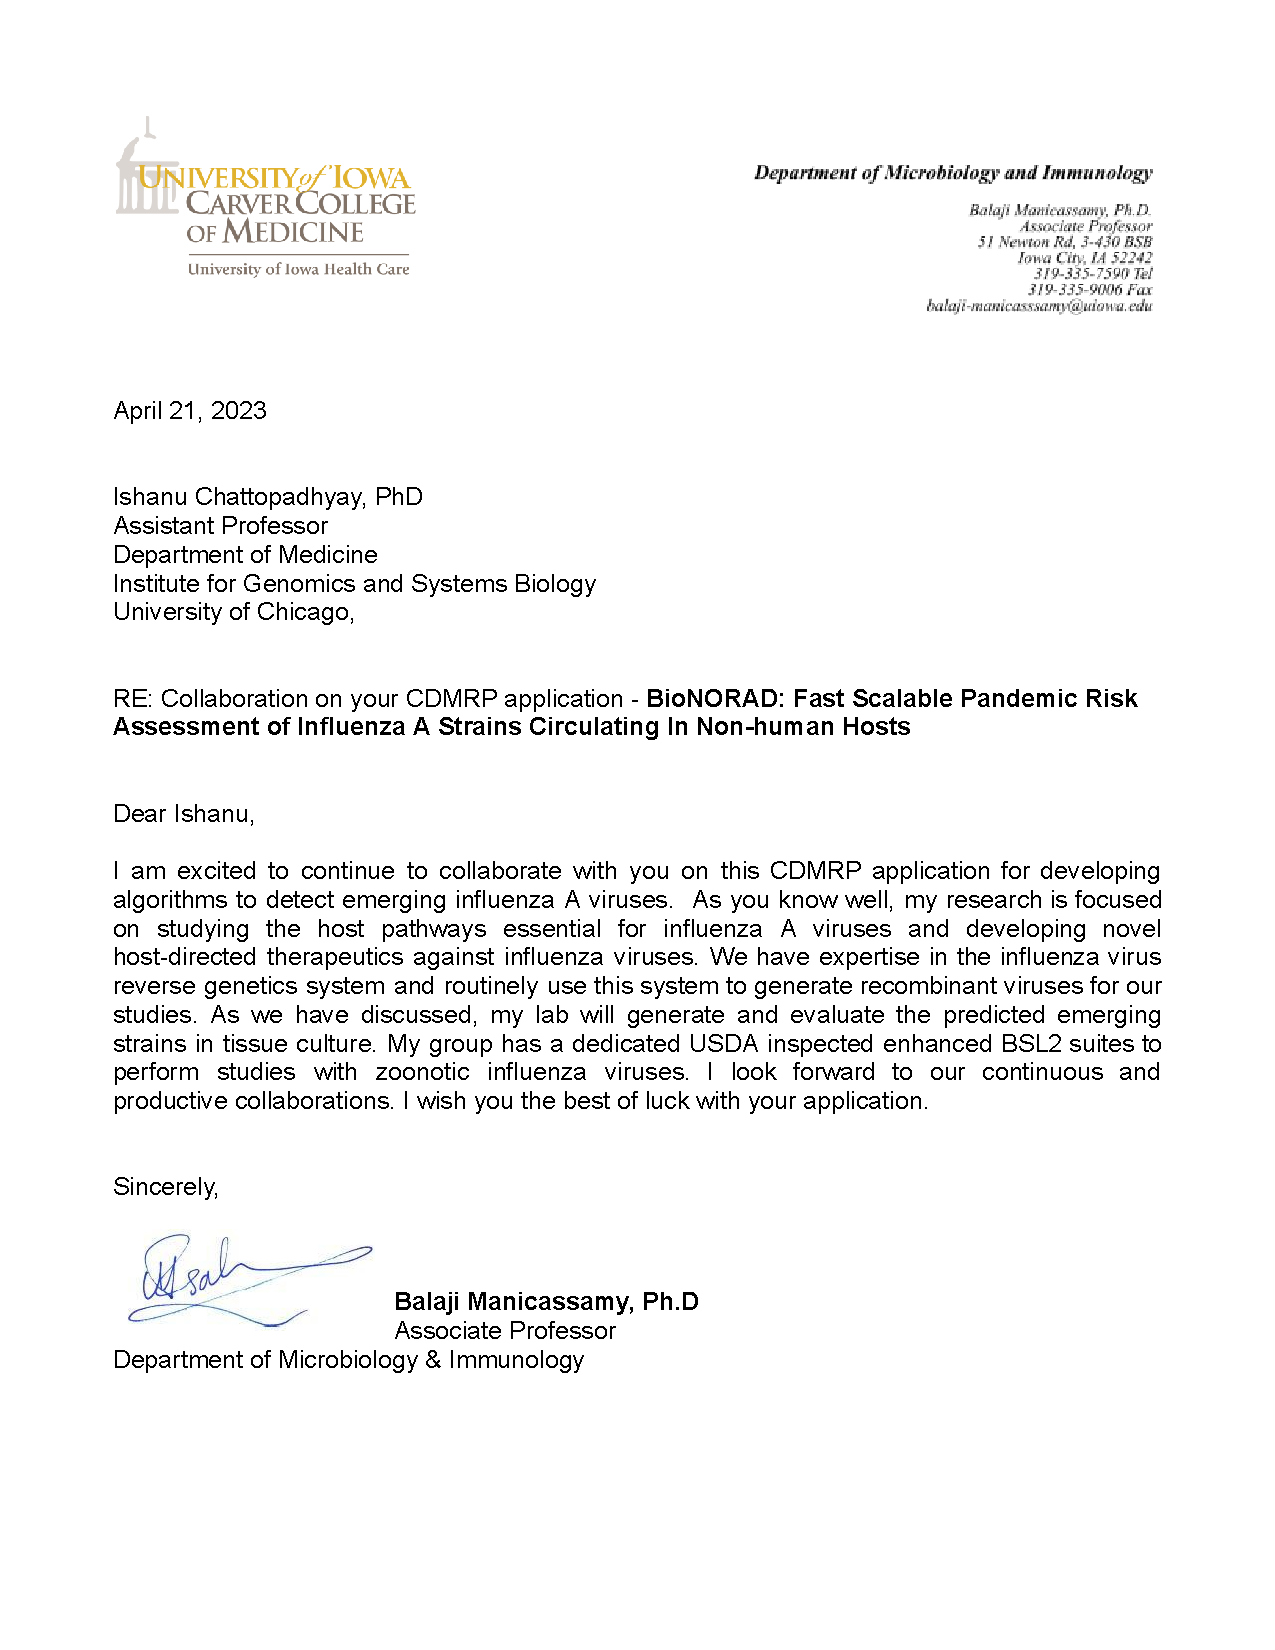
\includepdf[pages=-]{Figures/LOS-Manicassamy.pdf}


\clearpage
\setcounter{subsection}{0}
\section*{Intellectual and Material Property Plan}

\subsection{Intellectual Property (IP) Ownership and Management}
IP ownership \& management for the BioNORAD project will be governed by a formal agreement signed by all participating organizations specifying:
%
\begin{enumerate}
    \item Ownership of any existing IP (background IP), such as Chattopadhyay, I. (2022). ``Methods and systems for genomic based prediction of virus mutation'' (Patent No. WO2022108965A1). World Intellectual Property Organization. URL: \url{https://patents.google.com/patent/WO2022108965A1}, will be retained by the originating organization.
    \item New IP generated during the course of the project (foreground IP) will be jointly owned by the participating organizations, with the share of ownership determined by the contribution of each party to the development of the IP.
    \item The participating organizations will identify a designated IP representative who will be responsible for managing IP issues and ensuring compliance with the agreement.
    \item The  agreement will include provisions for resolving disputes related to IP ownership and management.
\end{enumerate}

\subsection{Licensing and Commercialization}
The participating organizations will develop a strategy for licensing and commercializing the foreground IP for the BioNORAD platform, considering the following factors:
\begin{enumerate}
    \item Evaluation of potential markets and applications for the platform, primarily focusing on global health organizations, governments, and pharmaceutical companies.
    \item Identification of potential licensees and strategic partners.
    \item Negotiation of licensing agreements, including royalties and other financial terms.
    \item Development of a patent strategy, including filing and maintenance of patents in relevant jurisdictions.
\end{enumerate}

\subsection{Commercialization Strategy}

\begin{enumerate}
    \item \textbf{Intellectual Property}: The participating organizations will develop and maintain a strong IP portfolio for the BioNORAD platform. This includes filing patent applications in key markets and ensuring that the IP is properly protected.
    \item \textbf{Market Size}: The target market for the developed technology will be global health organizations, governments, and pharmaceutical companies involved in pandemic prevention and response. This market is expected to grow significantly due to increasing awareness of pandemic risks and the need for proactive measures.
    \item \textbf{Financial Analysis}: The financial analysis will include a detailed assessment of the potential revenues, costs, and profitability of the BioNORAD platform. This will include projections for product pricing, market share, and revenue growth, as well as estimates of development costs, manufacturing expenses, and other operating costs.
    \item \textbf{Strengths and Weaknesses}: The commercialization plan will identify the platform's strengths and weaknesses, as well as opportunities and threats in the market. This analysis will help the participating organizations to strategically position the platform in the market and address potential challenges.
    \item \textbf{Barriers to the Market}: The commercialization plan will address potential barriers to market entry, such as competition, regulatory hurdles, and technology adoption challenges. Strategies will be developed to overcome these barriers and increase the chances of successful market penetration.
    \item \textbf{Competitors}: The commercialization plan will include an analysis of the competitive landscape, identifying key competitors and their strengths and weaknesses. This will help the participating organizations to differentiate the BioNORAD platform and develop a competitive advantage.
    \item \textbf{Management Team}: A strong management team will be assembled to lead the commercialization effort. This team will include individuals with experience in technology development, marketing, sales, and operations, as well as industry-specific expertise in pandemic prevention and response.
    \item \textbf{Significance and Timeline}: The commercialization plan will outline the significance of the BioNORAD platform in addressing the challenges of emerging pandemic threats and the need for proactive measures. A timeline for the development and commercialization of the technology will be provided, along with milestones to track progress and measure success.
\end{enumerate}
\subsection{Intellectual Products Expected}
\begin{enumerate}
[label=$\square$, leftmargin=0pt,
labelindent=0em, topsep=0.1em, labelsep=*, itemsep=.25em,itemindent=1em]\item Software implementations of \enet inference algorithm 
\item Generation of sequence data from the \enet models specying novel strains expected to arise in future
\item Patents filed by UChicago
\end{enumerate}
\subsection{Inventions and IP Rights at The University of Chicago}

\begin{figure}[t]
  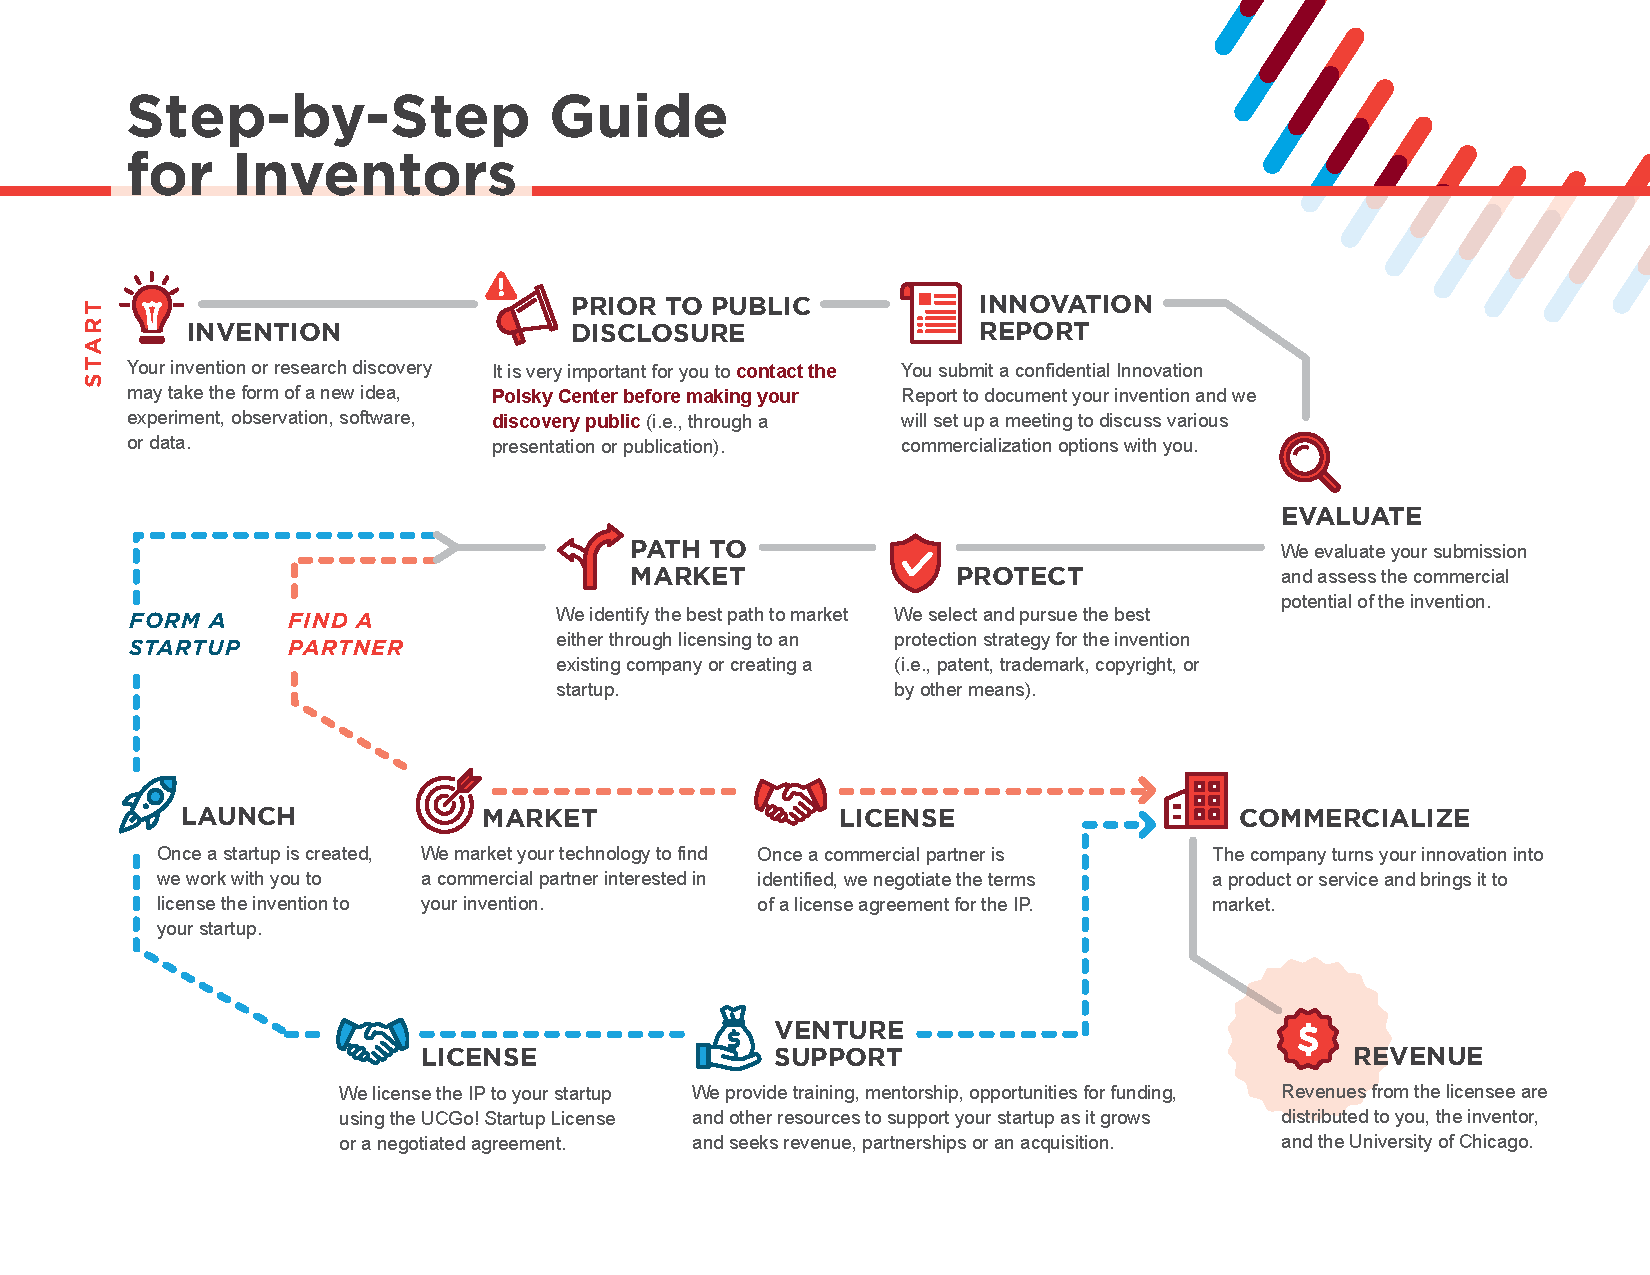
\includegraphics[width=\textwidth]{Figures/Polsky-Inventor-Pathway}

  \vspace{-35pt}
  
  \captionN{Inventor pathway to commercialization at the University of Chicago}\label{figPolsky}
\end{figure}

The University of Chicago is committed to the open and timely dissemination of research outcomes. Investigators in the proposed activity recognize that promising new methods, technologies, strategies and software programming may arise during the course of the research. The Investigators are aware of and agree to be guided by the principles for sharing research resources as described, for example, in the National Institutes of Health "Principles and Guidelines for Recipients of NIH Research Grants and Contracts on Obtaining and Disseminating Biomedical Research Resources".

While the investigators expect that research tools will be freely shared with the research community, opportunities for technology transfer through commercialization will be explored as appropriate. At the University of Chicago, its Polsky Center for Entrepreneurship and Innovation manages intellectual property (IP). The Polsky Center for Entrepreneurship and Innovation manages all technology transfer operations at the University of Chicago (See Figure~\ref{figPolsky}).

Our Polsky Science and Technology group serves as the central resource for transforming groundbreaking ideas and faculty discoveries into new products, services, and ventures. We have a dedicated team of scientists with deep technical expertise who are exclusively focused on managing intellectual property and negotiating partnerships and licenses for technologies developed by faculty, researchers, and staff. The Polsky Center serves faculty, staff and students by commercializing inventions, ideas and software developed at the University to ensure that new knowledge benefits society. Revenues from any commercial licenses will be shared with the inventor and reinvested in the research enterprise.



\clearpage

\section*{Data and Research Resources Sharing Plan}


The BioNORAD project aims to develop a platform for early identification and mitigation of emerging pandemic threats, particularly those caused by novel strains of influenza viruses. The project will generate several types of data and research resources that can be valuable to the scientific community. In this section, we describe how we plan to share these data and research resources  with the research community.

\subsection*{Types of Data and Research Resources}

The BioNORAD project will generate several types of data and research resources, including:

\begin{itemize}
    \item \textbf{Genomic data:} The project will generate predicted genomic sequences of key viral proteins of \infl.
    \item \textbf{Machine learning models:} The project will develop machine learning models for predicting the emergence and spread of novel strains of influenza viruses. These models will be based on the genomic  data acquired during the project from public sequence databases.
    \item \textbf{Software tools:} The project will develop software tools for analyzing genomic and clinical data, as well as for visualizing and interpreting the results of machine learning models. These tools will be valuable for researchers working on influenza viruses and other emerging infectious diseases.
\end{itemize}

\subsection*{Sharing Plan}

We plan to share the data and research resources generated by the BioNORAD project with the research community as widely as possible, while safeguarding the privacy of participants and protecting confidential and proprietary data and third-party intellectual property.

\subsubsection*{Data sharing}

We plan to deposit the genomic  data generated by the project in publicly accessible repositories with long-term DOI access. These repositories will provide a persistent and citable location for the data and ensure that they are discoverable and accessible to the research community. We will use the Zenodo platform to deposit the data, which will provide long-term archiving and DOI access. We will also ensure that the data are compliant with data sharing policies of funding agencies such as the National Institutes of Health and the Department of Defense. Genomic sequence data will be also deposited to NCBI. 

\subsubsection*{Model sharing}

We plan to deposit the machine learning models developed during the project in public repositories such as GitHub, with open-source licenses, making them freely available to the research community. We will provide documentation and instructions for running the models, as well as sample data for testing and validation. We will also encourage the research community to contribute to the development of the models by providing feedback and suggesting improvements.

\subsubsection*{Software sharing}

We plan to deposit the software tools developed during the project in public repositories such as GitHub, with open-source licenses, making them freely available to the research community. We will provide documentation and instructions for using the tools, as well as sample data for testing and validation. We will also encourage the research community to contribute to the development of the tools by providing feedback and suggesting improvements.

\subsection*{Feasibility and Appropriateness}

The data generated from this project will be shared through various channels to ensure maximum accessibility to the research community. In addition to depositing the software in a GitHub repository, models and data will be deposited in Zenodo, an open-access repository for scientific data, with a long-term DOI access. The datasets generated will be organized and labeled appropriately to enable easy retrieval, interpretation, and reuse by other researchers. The datasets will be accompanied by comprehensive documentation, including descriptions of the methods and procedures used to generate the data, as well as any relevant metadata.

To further facilitate the sharing of data and resources, the project team will follow best practices for data management, including adhering to FAIR (Findable, Accessible, Interoperable, Reusable) data principles. These practices include using standardized data formats and metadata, creating clear documentation for data and code, and ensuring that data and code are appropriately versioned and stored in secure and reliable repositories.

The project team recognizes that data sharing carries certain risks, particularly regarding the protection of sensitive information. However such risk is minimal in this project, which will not involve any clinical information or human participants.

In summary, the BIONORAD project is committed to promoting data and research resource sharing to enhance collaboration and accelerate the translation of research results into practical applications. The project team will ensure that data and resources generated during the project's period of performance are made widely available while safeguarding the any  proprietary information that we may use (including sequence data that do not carry permission to be posted publicly). By sharing and leveraging data and resources, this project will contribute to a more expeditious translation of research results into knowledge, products, and procedures to improve military health and global health security.

 \subsection*{Implementation in a Dual-Use Capacity}

 The knowledge, information, products, technologies, or applications gained from the proposed research could be implemented in a dual-use capacity to benefit the civilian population that also addresses a need related to military health. The research findings will be published in peer-reviewed journals, presented at scientific conferences, and disseminated to the research community. The findings will also be communicated to the wider community through various media, such as press releases, newsletters, and social media platforms. The knowledge generated by this research will have broad applications beyond the military, with potential benefits for the civilian population, including the development of vaccines, diagnostic tools, and treatments for infectious diseases.

 In summary, we will make every effort to ensure that all data and research resources generated during the project's period of performance will be made publicly available while safeguarding the privacy of participants and protecting confidential and proprietary data and third-party intellectual property. We recognize that the unique data generated by our project will be valuable to the research community, and we will make every effort to share this data with the research community. The research resources generated during the project will also be made publicly available. The knowledge, information, products, technologies, or applications gained from the research could be implemented in a dual-use capacity to benefit the civilian population that also addresses a need related to military health.

\clearpage

%\clearpage
%\section*{Public Health Service (PHS) Inclusion Enrollment Report}




%\clearpage
%\section*{Representations}




\clearpage

%\bibliographystyle{plainnat}
%\bibliography{asdgenenew}
\bibliographystyle{naturemag}
\bibliography{allbib}


\end{document}

